\documentclass{ximera}

 

\usepackage{epsfig}

\graphicspath{
  {./}
  {figures/}
}

\usepackage{morewrites}
\makeatletter
\newcommand\subfile[1]{%
\renewcommand{\input}[1]{}%
\begingroup\skip@preamble\otherinput{#1}\endgroup\par\vspace{\topsep}
\let\input\otherinput}
\makeatother

\newcommand{\includeexercises}{\directlua{dofile("/home/jim/linearAlgebra/laode/exercises.lua")}}

%\newcounter{ccounter}
%\setcounter{ccounter}{1}
%\newcommand{\Chapter}[1]{\setcounter{chapter}{\arabic{ccounter}}\chapter{#1}\addtocounter{ccounter}{1}}

%\newcommand{\section}[1]{\section{#1}\setcounter{thm}{0}\setcounter{equation}{0}}

%\renewcommand{\theequation}{\arabic{chapter}.\arabic{section}.\arabic{equation}}
%\renewcommand{\thefigure}{\arabic{chapter}.\arabic{figure}}
%\renewcommand{\thetable}{\arabic{chapter}.\arabic{table}}

%\newcommand{\Sec}[2]{\section{#1}\markright{\arabic{ccounter}.\arabic{section}.#2}\setcounter{equation}{0}\setcounter{thm}{0}\setcounter{figure}{0}}

\newcommand{\Sec}[2]{\section{#1}}

\setcounter{secnumdepth}{2}
%\setcounter{secnumdepth}{1} 

%\newcounter{THM}
%\renewcommand{\theTHM}{\arabic{chapter}.\arabic{section}}

\newcommand{\trademark}{{R\!\!\!\!\!\bigcirc}}
%\newtheorem{exercise}{}

\newcommand{\dfield}{{\sf dfield9}}
\newcommand{\pplane}{{\sf pplane9}}

\newcommand{\EXER}{\section*{Exercises}}%\vspace*{0.2in}\hrule\small\setcounter{exercise}{0}}
\newcommand{\CEXER}{}%\vspace{0.08in}\begin{center}Computer Exercises\end{center}}
\newcommand{\TEXER}{} %\vspace{0.08in}\begin{center}Hand Exercises\end{center}}
\newcommand{\AEXER}{} %\vspace{0.08in}\begin{center}Hand Exercises\end{center}}

% BADBAD: \newcommand{\Bbb}{\bf}

\newcommand{\R}{\mbox{$\Bbb{R}$}}
\newcommand{\C}{\mbox{$\Bbb{C}$}}
\newcommand{\Z}{\mbox{$\Bbb{Z}$}}
\newcommand{\N}{\mbox{$\Bbb{N}$}}
\newcommand{\D}{\mbox{{\bf D}}}
\usepackage{amssymb}
%\newcommand{\qed}{\hfill\mbox{\raggedright$\square$} \vspace{1ex}}
%\newcommand{\proof}{\noindent {\bf Proof:} \hspace{0.1in}}

\newcommand{\setmin}{\;\mbox{--}\;}
\newcommand{\Matlab}{{M\small{AT\-LAB}} }
\newcommand{\Matlabp}{{M\small{AT\-LAB}}}
\newcommand{\computer}{\Matlab Instructions}
\newcommand{\half}{\mbox{$\frac{1}{2}$}}
\newcommand{\compose}{\raisebox{.15ex}{\mbox{{\scriptsize$\circ$}}}}
\newcommand{\AND}{\quad\mbox{and}\quad}
\newcommand{\vect}[2]{\left(\begin{array}{c} #1_1 \\ \vdots \\
 #1_{#2}\end{array}\right)}
\newcommand{\mattwo}[4]{\left(\begin{array}{rr} #1 & #2\\ #3
&#4\end{array}\right)}
\newcommand{\mattwoc}[4]{\left(\begin{array}{cc} #1 & #2\\ #3
&#4\end{array}\right)}
\newcommand{\vectwo}[2]{\left(\begin{array}{r} #1 \\ #2\end{array}\right)}
\newcommand{\vectwoc}[2]{\left(\begin{array}{c} #1 \\ #2\end{array}\right)}

\newcommand{\ignore}[1]{}


\newcommand{\inv}{^{-1}}
\newcommand{\CC}{{\cal C}}
\newcommand{\CCone}{\CC^1}
\newcommand{\Span}{{\rm span}}
\newcommand{\rank}{{\rm rank}}
\newcommand{\trace}{{\rm tr}}
\newcommand{\RE}{{\rm Re}}
\newcommand{\IM}{{\rm Im}}
\newcommand{\nulls}{{\rm null\;space}}

\newcommand{\dps}{\displaystyle}
\newcommand{\arraystart}{\renewcommand{\arraystretch}{1.8}}
\newcommand{\arrayfinish}{\renewcommand{\arraystretch}{1.2}}
\newcommand{\Start}[1]{\vspace{0.08in}\noindent {\bf Section~\ref{#1}}}
\newcommand{\exer}[1]{\noindent {\bf \ref{#1}}}
\newcommand{\ans}{}
\newcommand{\matthree}[9]{\left(\begin{array}{rrr} #1 & #2 & #3 \\ #4 & #5 & #6
\\ #7 & #8 & #9\end{array}\right)}
\newcommand{\cvectwo}[2]{\left(\begin{array}{c} #1 \\ #2\end{array}\right)}
\newcommand{\cmatthree}[9]{\left(\begin{array}{ccc} #1 & #2 & #3 \\ #4 & #5 &
#6 \\ #7 & #8 & #9\end{array}\right)}
\newcommand{\vecthree}[3]{\left(\begin{array}{r} #1 \\ #2 \\
#3\end{array}\right)}
\newcommand{\cvecthree}[3]{\left(\begin{array}{c} #1 \\ #2 \\
#3\end{array}\right)}
\newcommand{\cmattwo}[4]{\left(\begin{array}{cc} #1 & #2\\ #3
&#4\end{array}\right)}

\newcommand{\Matrix}[1]{\ensuremath{\left(\begin{array}{rrrrrrrrrrrrrrrrrr} #1 \end{array}\right)}}

\newcommand{\Matrixc}[1]{\ensuremath{\left(\begin{array}{cccccccccccc} #1 \end{array}\right)}}



\renewcommand{\labelenumi}{\theenumi)}
\newenvironment{enumeratea}%
{\begingroup
 \renewcommand{\theenumi}{\alph{enumi}}
 \renewcommand{\labelenumi}{(\theenumi)}
 \begin{enumerate}}
 {\end{enumerate}\endgroup}



\newcounter{help}
\renewcommand{\thehelp}{\thesection.\arabic{equation}}

%\newenvironment{equation*}%
%{\renewcommand\endequation{\eqno (\theequation)* $$}%
%   \begin{equation}}%
%   {\end{equation}\renewcommand\endequation{\eqno \@eqnnum
%$$\global\@ignoretrue}}

%\input{psfig.tex}

\author{Martin Golubitsky and Michael Dellnitz}

%\newenvironment{matlabEquation}%
%{\renewcommand\endequation{\eqno (\theequation*) $$}%
%   \begin{equation}}%
%   {\end{equation}\renewcommand\endequation{\eqno \@eqnnum
% $$\global\@ignoretrue}}

\newcommand{\soln}{\textbf{Solution:} }
\newcommand{\exercap}[1]{\centerline{Figure~\ref{#1}}}
\newcommand{\exercaptwo}[1]{\centerline{Figure~\ref{#1}a\hspace{2.1in}
Figure~\ref{#1}b}}
\newcommand{\exercapthree}[1]{\centerline{Figure~\ref{#1}a\hspace{1.2in}
Figure~\ref{#1}b\hspace{1.2in}Figure~\ref{#1}c}}
\newcommand{\para}{\hspace{0.4in}}

\renewenvironment{solution}{\suppress}{\endsuppress}

\ifxake
\newenvironment{matlabEquation}{\begin{equation}}{\end{equation}}
\else
\newenvironment{matlabEquation}%
{\let\oldtheequation\theequation\renewcommand{\theequation}{\oldtheequation*}\begin{equation}}%
  {\end{equation}\let\theequation\oldtheequation}
\fi

\makeatother


\title{c18.tex}

\begin{document}
\begin{abstract}
BADBAD
\end{abstract}
\maketitle

\chapter{Numerical Solutions of ODEs}
\label{ch:NumSolODE}

\normalsize

In general it is difficult, if not impossible, to find solutions to 
differential equations analytically.   When this happens we rely on the
numerical approximation of solutions, and in this chapter we discuss 
how numerical solutions to initial value 
problems\index{initial value problem!numerical solution} of the form
\arraystart
\[
\begin{array}{rcl}
\dps\frac{dx}{dt}(t) & = & f(t,x(t)) \\
x(t_0) & = & x_0
\end{array}
\]
\arrayfinish
are found.  This will provide insight into the numerical
techniques used in the \Matlab programs {\sf dfield5},
{\sf pline} and {\sf pplane5}.

The numerical schemes that we consider approximate 
solutions up to a specified accuracy, and
in Section~\ref{sec:DNM} we describe the basic ideas
underlying the construction of such schemes.  In this
section we will see that in general there is an error between 
the numerical approximation and the analytic solution
of the underlying initial value problem.  One of the main
tasks in the numerical analysis of ODEs is to derive bounds
on this error, and in Section~\ref{sec:EEEM} we derive these bounds
for the simplest numerical scheme, {\em Euler's method}.  Finally, 
in Section~\ref{sec:LGEE}
we generalize this treatment and indicate how to derive error 
bounds for arbitrary numerical schemes.  In particular it
turns out that in general the {\em fourth order Runge-Kutta method\/}
leads to much more accurate numerical approximations than 
does Euler's method.


\section{A Description of Numerical Methods}
\label{sec:DNM}

By definition, derivatives are limits of Newtonian quotients and 
approximating this limit provides one of the basic ideas in the 
construction of numerical methods.  More precisely, let $x$ be the 
solution of the initial value problem $\dot x = f(t,x)$, $x(t_0)=x_0$.  
The derivative of $x$ at time $t$ is the limit
\[
\frac{dx}{dt}(t) = \lim_{h\to 0} \frac{x(t+h) - x(t)}{h}.
\]
Hence we expect
\begin{equation}  \label{eq:eul1}
x(t+h) \approx x(t) + h \frac{dx}{dt}(t) = x(t) + h f(t,x(t))
\end{equation}
to be a good approximation of $x$ at time $t+h$ for small $h$.
Indeed, by Taylor's formula
\arraystart
\begin{equation}\label{eq:tfeul}
\begin{array}{rcl}
\dps x(t+h)&=&
\dps x(t)+h\frac{dx}{dt}(t)+\frac{h^2}{2}\frac{d^2x}{dt^2}(t+\theta h)\\
&=& \dps x(t)+hf(t,x(t))+\frac{h^2}{2}\frac{d^2x}{dt^2}(t+\theta h),
\end{array}
\end{equation}
\arrayfinish
with an appropriate $0<\theta<1$.  Thus, the error made in the
approximation in \Ref{eq:eul1} is the size $h^2$
as long as the second derivative of $x(t)$ is bounded.
Consequently, if we know the value of the solution $x$ at time $t$, 
then we can use the right hand side $f$ in the differential equation 
to compute an approximation of the solution $x$ at time $t+h$.

\subsection*{Euler's Method} \index{Euler's method}
\index{Euler's method!explicit}

Since $f(t,x(t))$ is the derivative of $x$ at time $t$,
there is a simple geometric interpretation of \Ref{eq:eul1}
(see Figure~\ref{fig:eul1ill}).  Recall that the tangent line to the 
graph of the function $x(t)$ at the point $(t,x(t))$ is the line 
going through the point $(t,x(t))$ whose slope is $\dot{x}(t)=f(t,x(t))$.  
The approximation of $x$ at time $t+h$ is just the one given by the value 
of that tangent line at $t+h$.  The numerical method that is based on 
\Ref{eq:eul1} is called {\em Euler's method}.
It seems evident that smaller values of $h$ should lead to a more 
accurate approximation of the solution $x$ on the interval
$[t,t+h]$.  On the other hand, note that simultaneously the 
length of the interval $[t,t+h]$ is shrinking and that more
approximations are needed to approximate a solution on a
fixed time interval.
\begin{figure}[htb]
   \centerline{%
   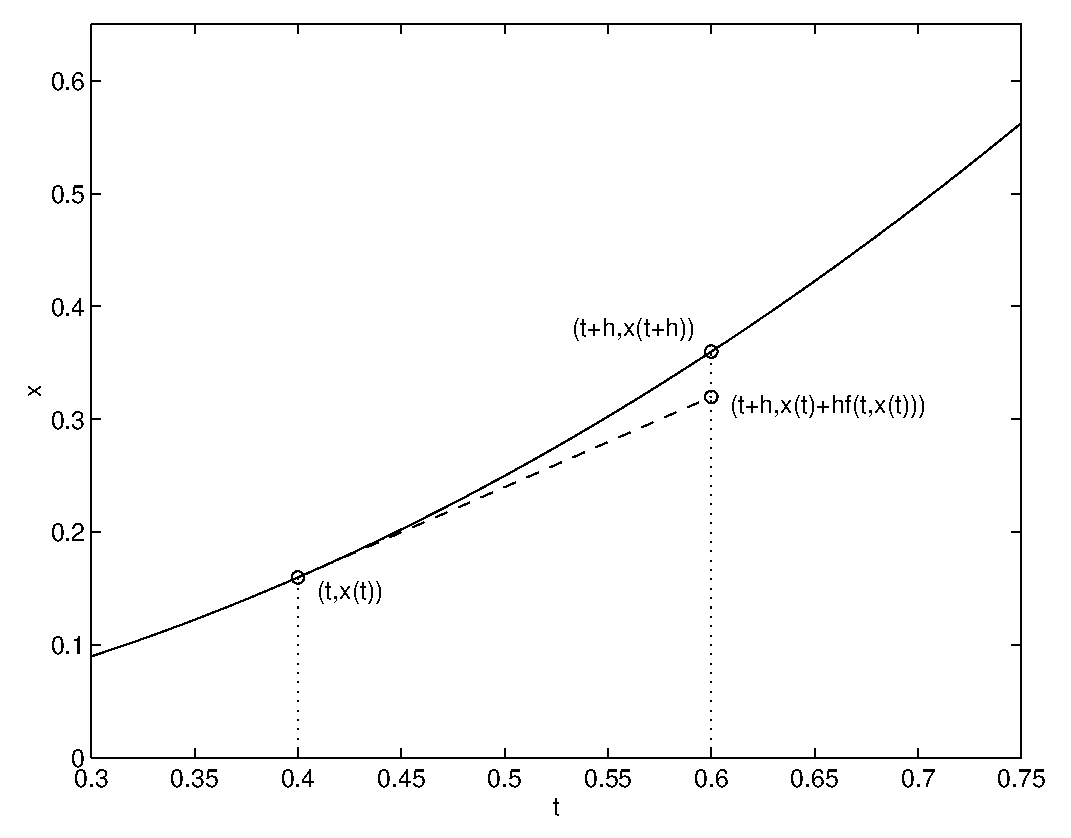
\psfig{file=figures/eul1.eps,width=4.6in}}
   \caption{Illustration of one step in Euler's method
   for $h=0.2$.}
   \label{fig:eul1ill}
\end{figure}

Concretely, Euler's method produces a sequence of approximations
to a solution of an initial value problem.  To understand this point, 
begin the numerical integration at the exact initial value $(t_0,x_0)$.  
Choose a {\em step size\/} \index{step size}
$h>0$.  Use \Ref{eq:eul1} to obtain after 
one {\em integration step\/} \index{integration step}
the approximation $x(t_1)\approx x_1$ where
\[
t_1 = t_0+h \AND x_1 = x_0 + h f(t_0, x_0).
\]
Continuing this process, construct a sequence
\begin{equation}  \label{eq:eulmethod}
t_{k+1} = t_k+h \AND x_{k+1} = x_k + h f(t_k, x_k)
\end{equation}
for $k=0,1,\ldots,K-1$ where $K$ is the total number of 
steps that are performed in the numerical approximation.

\subsubsection*{An Example of Euler's Method}
We illustrate how Euler's method works for the example
\arraystart
\begin{equation}  \label{eq:eulexivp}
\begin{array}{rcl}
\dps\frac{dx}{dt} & = & x+t\\
  x(1) & = & 2,
\end{array}
\end{equation}
\arrayfinish
by using \Matlab to compute an approximation to $x(3)$.  Suppose that we
set the step size to $h = 0.2$.  Then the number of steps needed to reach 
$t=3$ is $K=10$.  The code for computing the sequence in 
\Ref{eq:eulmethod} is:

\begin{verbatim}
h    = 0.2;
t(1) = 1;
x(1) = 2;
K    = 10;
for k = 1:K
   t(k+1) = t(k)+h;
   x(k+1) = x(k)+h*(x(k)+t(k));
end
plot(t,x,'o')
hold on
plot(t,x,'--')
xlabel('(a)')
\end{verbatim}\index{\computer!for\ldots end}\index{\computer!plot}
\index{\computer!hold}
The result is shown in Figure~\ref{fig:eulex1}(a).  Note that the
{\sf 'o'} in the \Matlab command {\tt plot(t,x,'o')} puts o's at the 11 
numerically computed points and the {\sf '-\,-'} in the command
{\tt plot(t,x,'--')} interpolates dashed lines between successive o's. 
Moreover, the statements within the {\tt for} loop --- that is the
lines from {\tt for k = 1:K} up to the {\tt end} --- 
reproduce the iteration procedure given in \Ref{eq:eulmethod}.
(In \Matlab the index of a vector is not allowed to be zero. Therefore, 
the {\tt for} loop is programmed to run from $k=1,\ldots,K$ rather than 
from $k=0,\ldots,K-1$.)

\subsubsection*{Comparison of Numerical Solutions with Exact Solutions}
\index{solution!numerical}\index{solution!exact}

We now compare the numerical approximation with the exact solution 
of \Ref{eq:eulexivp}, that is given by
\[
x(t) = 4e^{t-1}-t-1.
\]
This comparison is made in Figure~\ref{fig:eulex1}(b).  The second
curve in the figure is obtained using the additional commands
\begin{verbatim}
s = 1 : 0.01 : 3;
y = 4*exp(s-1)-s-1;  
plot(s,y)        
xlabel('(b)')
\end{verbatim}
Note that in that figure the scale on the vertical axis is
different from the one in Figure~\ref{fig:eulex1}(a).
\begin{figure}[htb]
   \centerline{%
   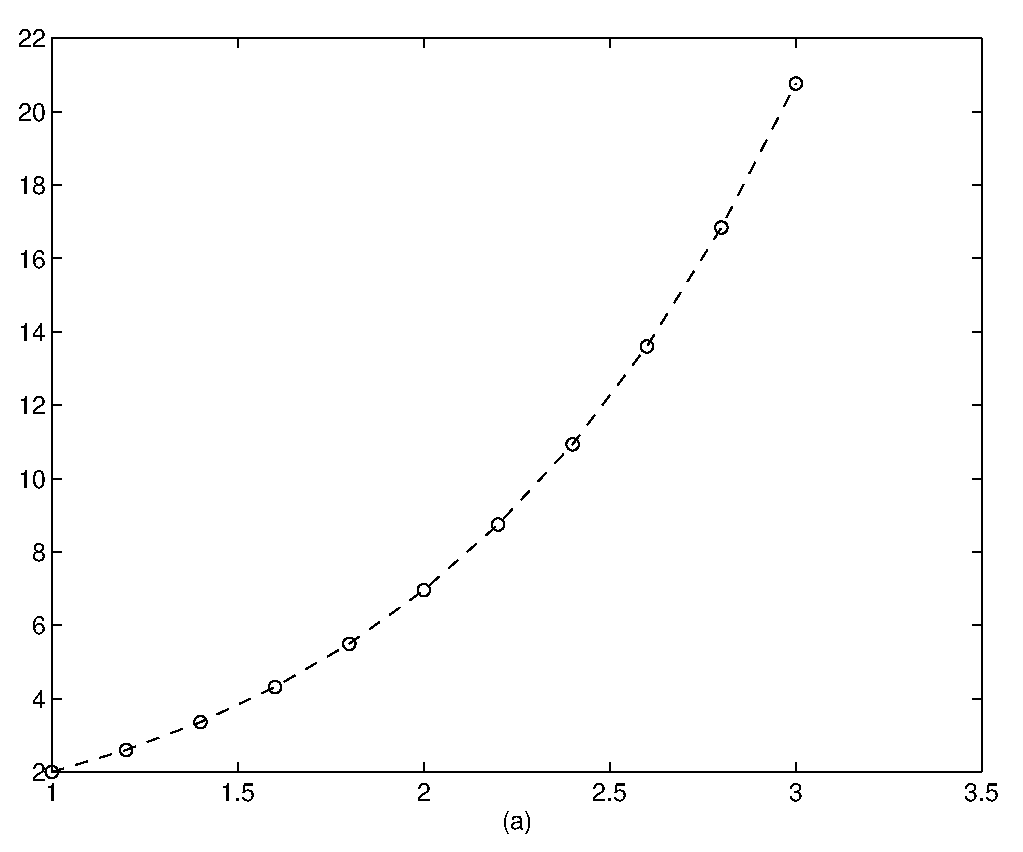
\psfig{file=figures/eulex1.eps,width=3in}
   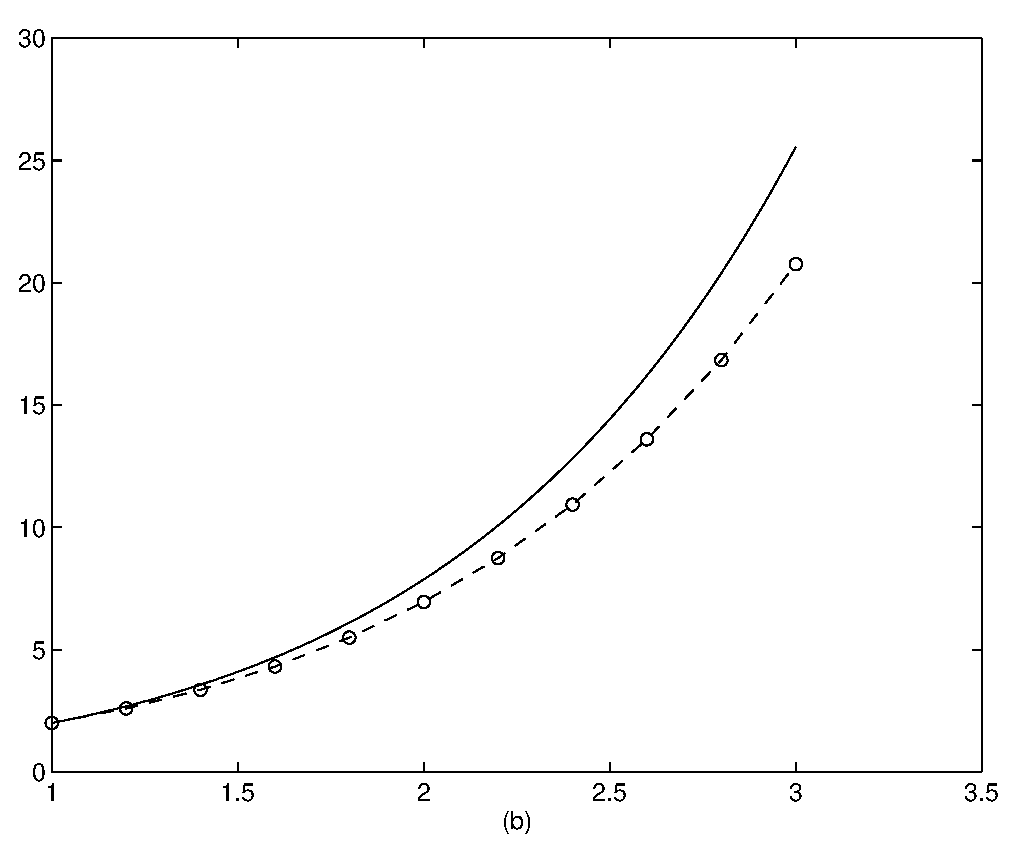
\psfig{file=figures/eulex2.eps,width=3in}}
   \caption{Approximation of the solution of 
   \protect\Ref{eq:eulexivp} by Euler's method.  
   (a) Circles mark the computed points; dashed lines 
    are linear interpolations between the o's.  (b)  A comparison is 
    made to the exact solution pictured as a solid line.}
   \label{fig:eulex1}
\end{figure}


In this example we see that after just $10$ steps the numerical solution 
of the initial value problem\index{initial value problem!numerical solution} 
by Euler's method has led to a significant 
error (see Figure~\ref{fig:eulex1} (b)).  There are two ways to proceed.
Either we can use a smaller step size\index{step size} in 
Euler's method in an attempt to 
improve accuracy or we can develop numerical methods that give more 
precise results for the same step size. For an illustration of the
first approach we show in Figure~\ref{fig:eulimpr}
an approximation with Euler's method using a step size
$h=0.05$.  It can be seen that the error is now indeed much smaller
but that also quite a few iterations of Euler's method are needed 
to produce this result.  Therefore the latter approach has 
generally proved preferable and one idea for improving accuracy is 
to replace $f(t_k,x_k)$ in the right hand side of 
\Ref{eq:eulmethod} by another expression in ways that we now explain.
\begin{figure}[htb]
   \centerline{%
   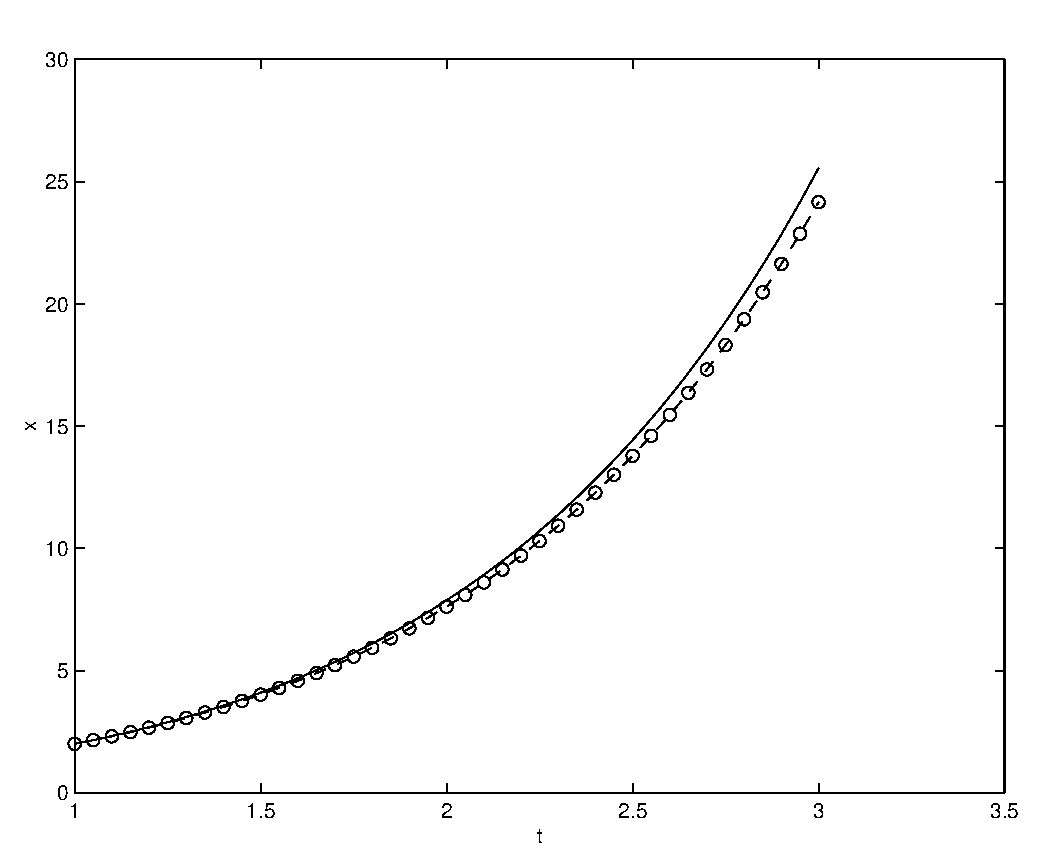
\psfig{file=figures/eulimpr.eps,width=3.4in}}
   \caption{Approximation of the solution of
   \protect\Ref{eq:eulexivp} by Euler's method with step size
   $h=0.05$.  (Marks and lines as in Figure~\protect\ref{fig:eulex1}.)}
   \label{fig:eulimpr}
\end{figure}


\subsection*{Implicit Methods}  

In Euler's method, the approximation $x_{k+1}$ is computed using the 
tangent line to the graph of the solution at the point $(t_k,x_k)$.  
Another idea is to approximate the graph of $x(t)$ by the line passing 
through the point $(t_k,x_k)$ whose slope is $f(t_{k+1},x_{k+1})$.  
This idea leads to the numerical approximation
\[
t_{k+1} = t_k+h \AND x_{k+1} = x_k + h f(t_{k+1}, x_{k+1})
\]
which is known as the {\em implicit Euler method}.  
\index{implicit Euler method} \index{Euler's method!implicit}
One difficulty with 
this method is that we do not yet know what the value of $x_{k+1}$ is.
However, it is {\em implicitly\/} defined in the sense that
we can think of the iteration step 
\begin{equation}
\label{eq:impleulit}
x_{k+1} = x_k + h f(t_{k+1}, x_{k+1})
\end{equation}
as an equation in the unknown $x_{k+1}$ and use this nonlinear equation 
to solve for $x_{k+1}$.  We remark that there are
ODEs (e.g.\ so-called {\em stiff\/} equations) for which implicit 
schemes typically produce more reliable results.  On the other hand, 
implicit methods require considerable additional numerical effort at 
each time step in order to solve the equations for $x_{k+1}$. 

An implicit numerical method that is more accurate than implicit Euler 
is obtained by just averaging the Euler and implicit Euler 
approximations, to obtain
\begin{equation}
\label{eq:imtrap}
t_{k+1} = t_k+h \AND x_{k+1} = x_k + \frac{h}{2}
\Big( f(t_k, x_k)+f(t_{k+1}, x_{k+1})\Big).
\end{equation}
This method is called the {\em implicit trapezoidal rule}.  
\index{implicit trapezoidal rule}

\subsection*{The Modified Euler Method} \index{modified Euler method}
\index{Euler's method!modified}

As we discussed, the problem with implicit methods is that they require
the solution of a nonlinear equation at each time step.  In principle
this can also be done numerically, but such solutions 
require much numerical effort.  This problem can partly be overcome by 
using a clever idea discovered by {\sc Runge} (1895).  We illustrate 
this idea on the implicit trapezoidal rule.  Rather than determining 
$x_{k+1}$ directly from \Ref{eq:imtrap}, first estimate 
$x_{k+1}$ by $y_{k+1}$ using Euler's 
(tangent line) method.  Then use the estimate $y_{k+1}$ in the implicit 
trapezoidal rule\index{implicit trapezoidal rule}.
In formulas we obtain:
\[
t_{k+1} = t_k+h \AND
\left\{\begin{array}{rcl}
y_{k+1} & = & x_k + h f(t_k, x_k)\\
x_{k+1} & = & x_k + \frac{h}{2}
\Big( f(t_k, x_k)+f(t_{k+1}, y_{k+1})\Big),
\end{array}\right.
\]
or, in one line,
\begin{equation}
\label{eq:meulmethod}
t_{k+1} = t_k+h \AND
x_{k+1} = x_k + \frac{h}{2}
\Big( f(t_k, x_k)+f(t_{k+1}, x_k + h f(t_k, x_k))\Big).
\end{equation}
The resulting numerical method is called the {\em modified Euler method}.
\index{modified Euler method} \index{Euler's method!modified}

Let us use \Matlab to solve the initial value problem
\index{initial value problem!numerical solution}
\Ref{eq:eulexivp} by the modified Euler method.  
Using the same data as in the previous example we type
\begin{verbatim}
h    = 0.2;
t(1) = 1;
x(1) = 2;
K    = 10;
for k = 1:K
   t(k+1) = t(k)+h;
   y(k)   = x(k)+h*(x(k)+t(k));
   x(k+1) = x(k)+(h/2)*(x(k)+t(k)+y(k)+t(k+1));
end
plot(t,x,'o')
hold on
plot(t,x,'--')
s = 1 : 0.01 : 3;
y = 4*exp(s-1)-s-1;
plot(s,y)
xlabel('(a)')
\end{verbatim}
to obtain the illustration in Figure~\ref{fig:mEul}(a).
We see that the approximation can hardly be distinguished from
the exact solution.  Even if we double the step size\index{step size} 
to $h=0.4$ and reduce the number of steps to $K=5$, the 
approximation is still acceptable.  See Figure~\ref{fig:mEul}(b).

\begin{figure}[htb]
   \centerline{%
   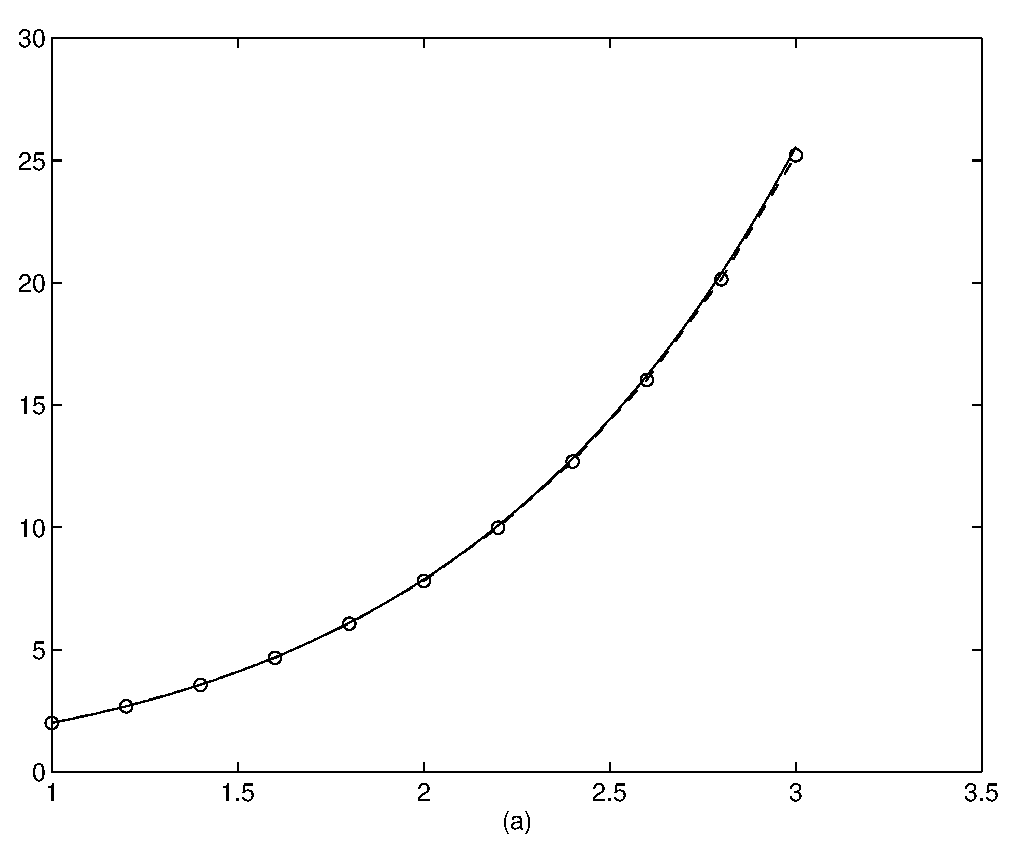
\psfig{file=figures/meul1.eps,width=3in}
   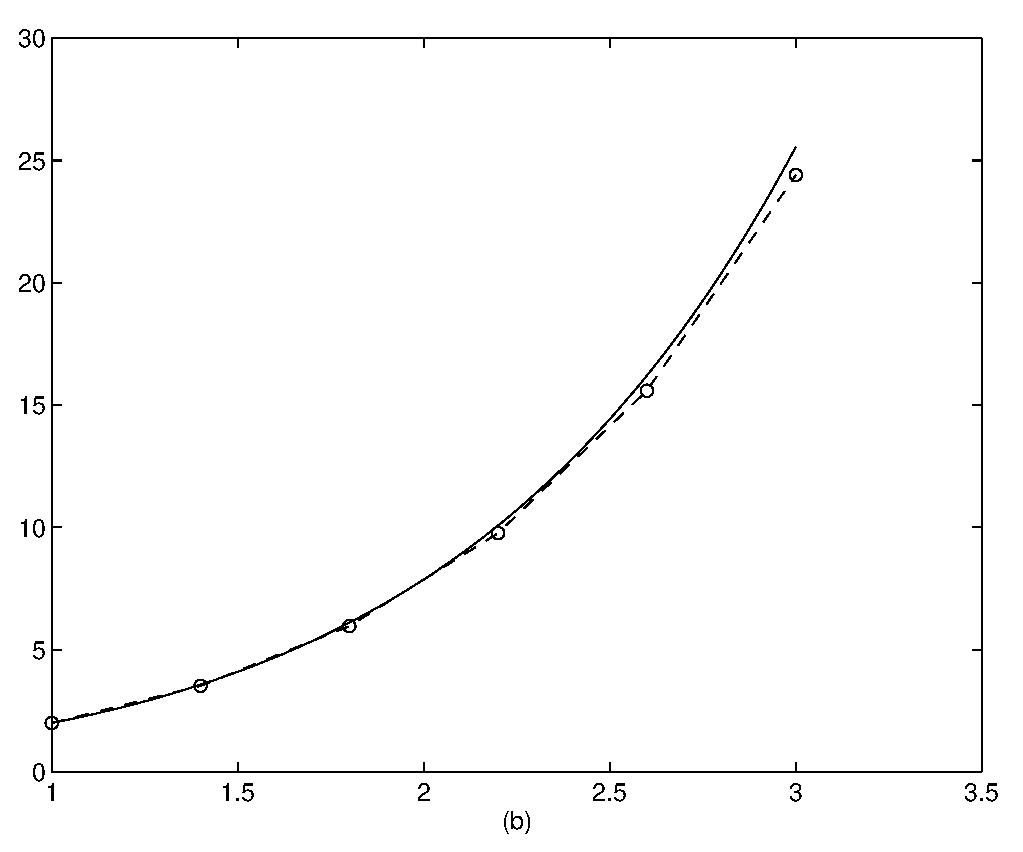
\psfig{file=figures/meul2.eps,width=3in}}
   \caption{Approximations of the solution of
   \protect\Ref{eq:eulexivp} by the modified Euler method
   with step sizes: (a) $h=0.2$; (b) $h=0.4$.
   The exact solution is shown with a solid line.}
   \label{fig:mEul}
\end{figure}

\subsection*{Fourth Order Runga-Kutta Method}
\index{fourth order Runge-Kutta method}
\index{Runge-Kutta method!fourth order}

The idea in the construction of the modified Euler method is to obtain a 
better approximation of the solution by using more information on the 
underlying differential equation.  This is realized in the scheme by 
taking the arithmetic average of two evaluations of the right hand side 
$f$ at different points rather than at just one point as in the 
standard Euler methods.

In the frequently used {\em fourth order Runge-Kutta method\/} four 
different evaluations of $f$ are taken into account in the computation of 
the next iterate.  The method is given as follows: set
\begin{eqnarray*}
f_1 &=& f(t_k,x_k)\\
f_2 &=& f\left(t_k+\frac{h}{2},x_k+\frac{h}{2}f_1\right)\\
f_3 &=& f\left(t_k+\frac{h}{2},x_k+\frac{h}{2}f_2\right)\\
f_4 &=& f(t_k+h,x_k+hf_3),
\end{eqnarray*}
and define the new approximation by
\[
x_{k+1} = x_k+\frac{h}{6}(f_1+2f_2+2f_3+f_4).
\]
By this method we can approximate solutions of differential equations
in a very precise way.  We illustrate this by an application to 
the initial value problem \Ref{eq:eulexivp}.  In Figure~\ref{fig:rk1} we
show the approximation obtained with the step size $h=0.6$ for $K=20$
steps.  The result is particularly convincing --- observe that
in contrast to Figures~\ref{fig:eulex1}--\ref{fig:mEul} the solution is
approximated on a significantly larger interval.
\begin{figure}[htb]
   \centerline{%
   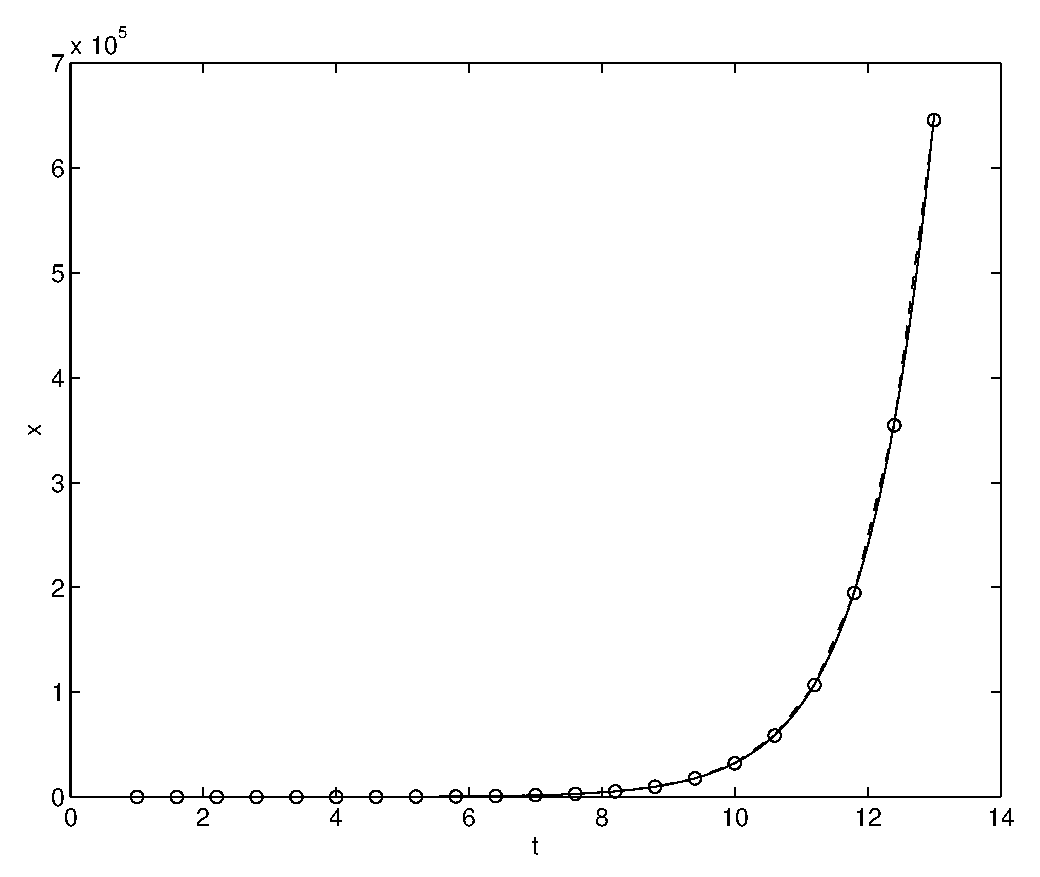
\psfig{file=figures/runkut1.eps,width=3.6in}}
   \caption{Approximation of the solution of
   \protect\Ref{eq:eulexivp} obtained by the fourth order Runge-Kutta
   method.  The exact solution is superimposed (solid line).}
   \label{fig:rk1}
\end{figure}

\subsection*{Systems of Differential Equations}

All the methods we have introduced in this section can
also be used to find numerically solutions of systems 
of differential equations.  We illustrate this fact for
systems of two equations using Euler's method.

In the scalar case the underlying idea for 
Euler's method\index{Euler's method} was 
to approximate the solution of the differential equation over 
a short interval by a line that is tangent to the solution curve
(see Figure~\ref{fig:eul1ill}).  We now use the same approach 
by applying this idea to each component of the solution.

Suppose that $(x(t),y(t))$ is a solution of the initial value problem
\arraystart
\begin{equation}
\label{eq:numanalsys}
\begin{array}{rcl}
\dps \frac{dx}{dt} & = & f(t,x,y)\\
\dps \frac{dy}{dt} & = & g(t,x,y),
\end{array}
\end{equation}
\arrayfinish
where $(x(t_0),y(t_0))= (x_0,y_0)$.  As in \Ref{eq:eul1}
we obtain for the components $x(t)$ and $y(t)$
by using the differential equation 
\begin{eqnarray*}
x(t+h) & \approx & x(t) + h \frac{dx}{dt}(t) = x(t) + h f(t,x(t),y(t))\\
y(t+h) & \approx & y(t) + h \frac{dy}{dt}(t) = y(t) + h g(t,x(t),y(t)).
\end{eqnarray*}
Again $h>0$ is called the step size\index{step size}.
We can now proceed as in the case of a scalar differential equation 
and obtain in analogy to \Ref{eq:eulmethod} 
\begin{eqnarray*}
t_{k+1} = t_k+h \AND 
\left\{\begin{array}{rcl}
x_{k+1} &=& x_k + h f(t_k,x_k,y_k)\\
y_{k+1} &=& y_k + h g(t_k,x_k,y_k)
\end{array}\right.
\quad (k=0,1,\ldots,K-1).
\end{eqnarray*}
Using vector notation Euler's method applied to the initial value problem
\Ref{eq:numanalsys} can be written as
\arraystart
\begin{equation}
\begin{array}{rcl}
\vectwo{x_{k+1}}{y_{k+1}} & = & 
\vectwo{x_k}{y_k} + h \vectwo{f(t_k,x_k,y_k)}{g(t_k,x_k,y_k)}\\
t_{k+1} & = & t_k + h,
\end{array}
\end{equation}
\arrayfinish
for $k=0,1,\ldots,K$.

Similarly, the implicit Euler 
method\index{Euler's method!implicit}\index{implicit Euler method} 
takes the form
\begin{eqnarray*}
\vectwo{x_{k+1}}{y_{k+1}} & = &  \vectwo{x_k}{y_k} + 
h \vectwo{f(t_{k+1},x_{k+1},y_{k+1})}{g(t_{k+1},x_{k+1},y_{k+1})}\\
t_{k+1} &=& t_k + h.
\end{eqnarray*}
Let us use \Matlab to compute an approximation of the initial
value problem
\arraystart
\begin{equation}
\label{eq:numanalex1}
\begin{array}{rcl}
\dps \frac{dx}{dt} & = & y-3t\\
\dps \frac{dy}{dt} & = & y+x^2,
\end{array}
\end{equation}
\arrayfinish
where $(x(1),y(1))= (0,2)$.  We specify the 
step size $h=0.05$ and find an approximation on the interval 
$[1,3]$ by typing
\begin{verbatim}
h    = 0.05;
t(1) = 1;
x(1) = 0;
y(1) = 2;
K    = 40;
for k = 1:K
   t(k+1) = t(k)+h;
   x(k+1) = x(k)+h*(y(k)-3*t(k));
   y(k+1) = y(k)+h*(y(k)+x(k)^2);
end
plot(x,y,'o')
hold on
plot(x,y,'--')
xlabel('x')
ylabel('y')
\end{verbatim}\index{\computer!for\ldots end}\index{\computer!plot}
\index{\computer!hold}
The result is shown in Figure~\ref{fig:sysEul1}.
\begin{figure}[htb]
   \centerline{%
   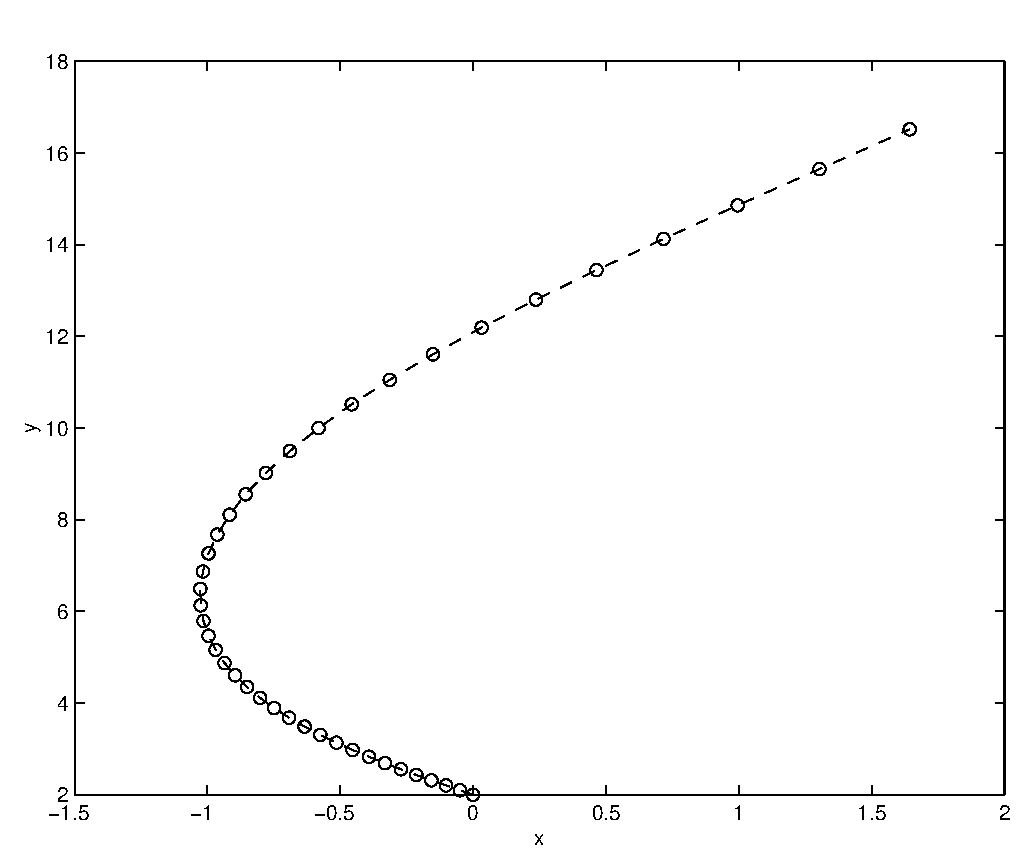
\psfig{file=figures/eulsys1.eps,width=3.6in}}
   \caption{Approximation of the solution of
   \protect\Ref{eq:numanalex1} by Euler's method
   with step size $h=0.05$.  The single points of
   the approximation are marked by circles.}
   \label{fig:sysEul1}
\end{figure}
Observe that the solution $(x(t),y(t))$ is graphed in
the $xy$-plane.
In particular, the variable $t$ does not appear in the figure 
and this is the reason why the single steps in the approximation
do not seem to be equally spaced.  However, in
Figure~\ref{fig:sysEul2} we show graphs of the approximations
of the time series $x$ vs.\ $t$ and $y$ vs.\ $t$. Here 
it can be seen that the step size is indeed constant.
\begin{figure}[htb]
   \centerline{%
   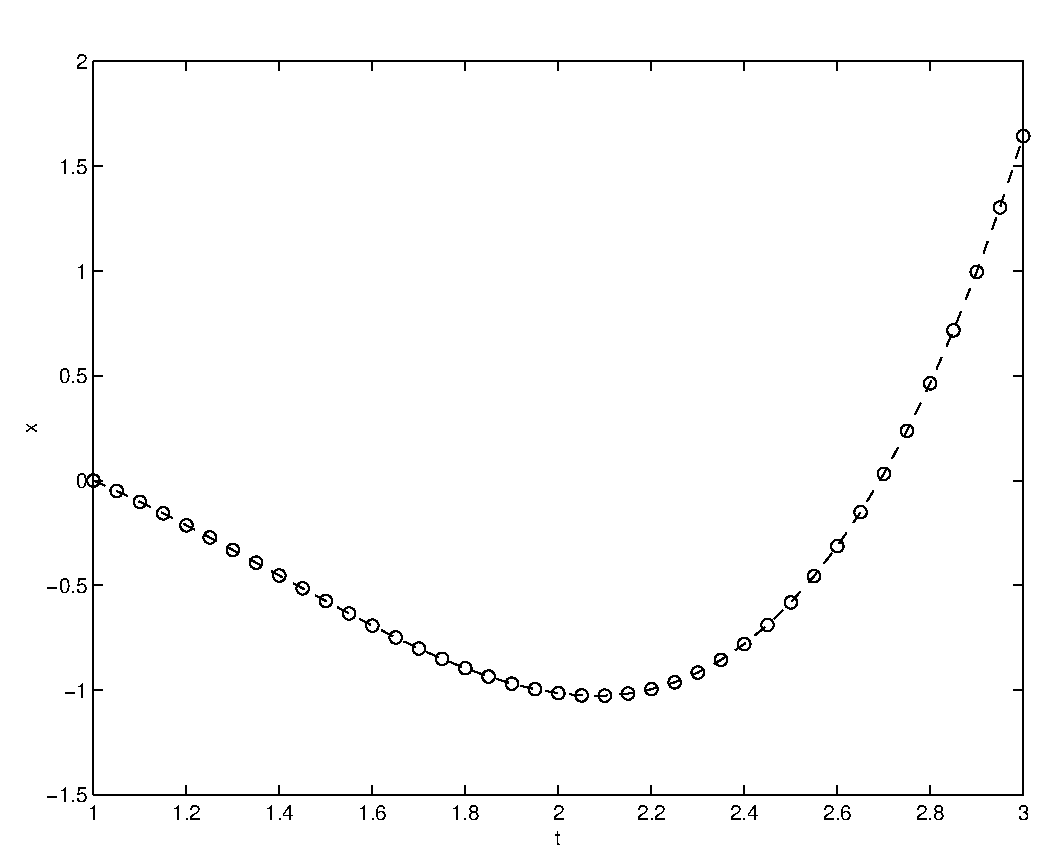
\psfig{file=figures/eulsys2.eps,width=3in}
   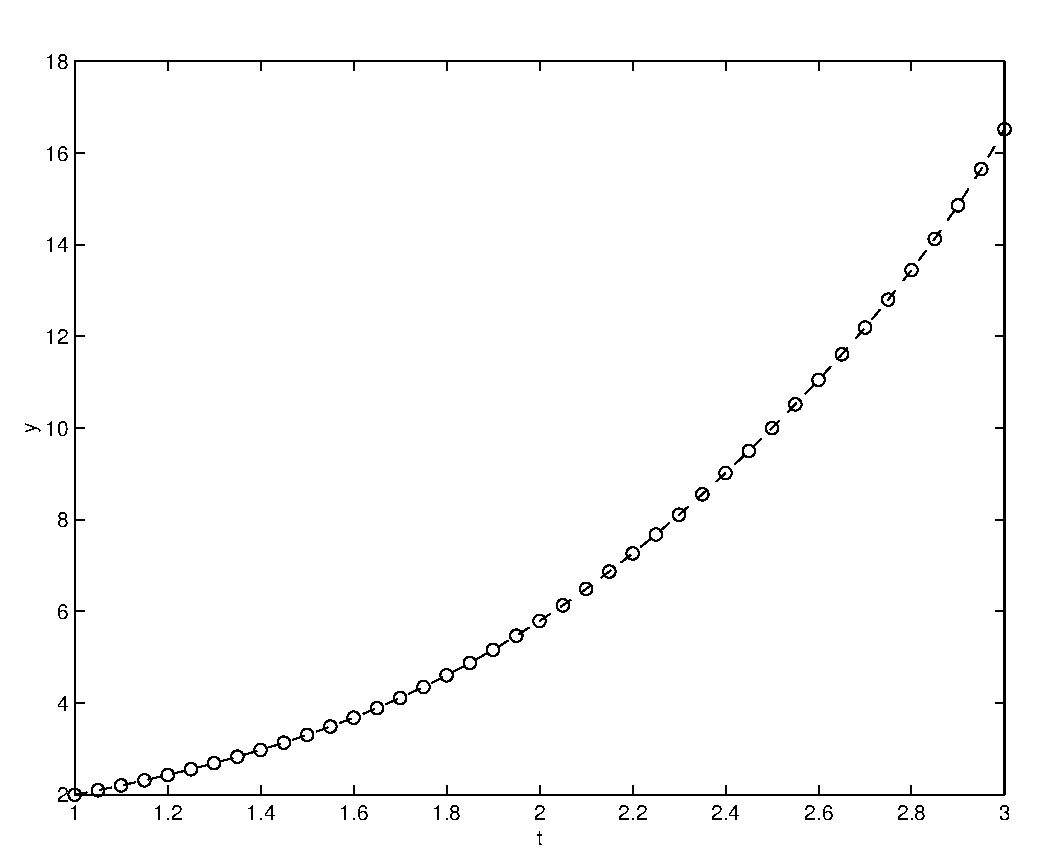
\psfig{file=figures/eulsys3.eps,width=3in}}
   \caption{Approximation of the $x$- and $y$-components
   of the solution of \protect\Ref{eq:numanalex1} by Euler's method
   with step size $h=0.05$.}
   \label{fig:sysEul2}
\end{figure}


There are several ways to improve the accuracy of 
numerical schemes approximating solutions of initial value problems. 
One very successful method is to adapt the step size $h$ in each
step of the numerical approximation.  We illustrate this
strategy in Appendix~\ref{sec:appslc}.


\subsection*{General Runga-Kutta Methods}
\index{Runge-Kutta method!general}

The modified Euler method as well as the fourth order Runge-Kutta
method are specific examples of a general class of 
numerical schemes for the solution of initial value 
problems\index{initial value problem!numerical solution}.
These schemes are called {\em Runge-Kutta methods}.  A general explicit 
Runge-Kutta method is fully described by numbers
\[
b_1,\ldots,b_s\AND c_1,\ldots,c_s,
\]
and 
\[
a_{pq}, \quad p=2,\ldots,s,\quad q=1,\ldots,p-1.
\]
With these numbers the $k^{th}$ step in the numerical solution of an 
initial value problem using a Runge-Kutta method can be described
as follows. Given $(t_k,x_k)$ first evaluate $f$ for $s$ times:
\begin{eqnarray*}
f_1 & = & f\left( t_k+c_1 h, x_k \right)\\
f_2 & = & f\left( t_k+c_2 h, x_k +ha_{21} f_1\right)\\
f_3 & = & f\left( t_k+c_3 h, x_k +h(a_{31} f_1 + a_{32} f_2)\right)\\
& \vdots &\\
f_s & = & f\left( t_k+c_s h, x_k +h\sum_{j=1}^{s-1}a_{ij} f_j\right).
\end{eqnarray*}
Second, obtain the next approximation by a weighted average
of $f_1,\ldots,f_s$:
\[
t_{k+1} = t_k+h \AND x_{k+1} = x_k + h\sum_{i=1}^s b_i f_i.
\]
We now show that --- except for the implicit schemes ---
all the methods that we have discussed are Runge-Kutta methods.

\begin{itemize}
\item[(a)] {\em Euler's method:} 
\index{Euler's method}
set
\[
s=1,\quad b_1=1,\quad c_1=0 
\]
and there are no $a_{pq}$'s.
\item[(b)] {\em The modified Euler method:} 
\index{modified Euler method} set
\[
s=2,\quad b_1=b_2=1/2,\quad c_1=0,\quad c_2=1,\quad a_{21}=1.
\]
Indeed, using these data
\begin{eqnarray*}
f_1 &=& f(t_k,x_k)\\
f_2 &=& f(t_{k+1},x_k+hf_1)=f(t_{k+1},x_k+hf(t_k,x_k)),
\end{eqnarray*}
and
\begin{eqnarray*}
x_{k+1} &=& x_k + h \left(\frac{1}{2}f_1 + \frac{1}{2}f_2\right)\\
&=& x_k + \frac{h}{2}
\Big( f(t_k, x_k)+f(t_{k+1}, x_k + h f(t_k, x_k))\Big).
\end{eqnarray*}
Hence we have obtained \Ref{eq:meulmethod}.
\item[(c)] {\em Fourth order Runge-Kutta method:} 
\index{fourth order Runge-Kutta method}
\index{Runge-Kutta method!fourth order}
set 
\[
s=4,\quad b_1=b_4=1/6,\quad b_2=b_3=2/6,\quad 
c_1=0,\quad c_2=c_3=1/2,\quad c_4=1,
\]
and 
\[
a_{21}=1/2,\quad a_{31}=0,\quad a_{32}=1/2,\quad
a_{41}=0,\quad a_{42}=0,\quad a_{43}=1.
\]
\end{itemize}


\EXER

\TEXER

\begin{exercise} \label{c15.1.1}
Consider the initial value problem
\[
\begin{array}{rcl}
\dps\frac{dx}{dt}(t) & = & -2 \\
x(t_0) & = & 0.
\end{array}
\]
Show that in this case an application of Euler's method 
leads to exact results for all step sizes $h$,
that is $x_k=x(t_k)$ for all $k$.
\end{exercise}

\begin{exercise} \label{c15.1.2}
Write down the implicit trapezoidal rule for the initial
value problem \Ref{eq:numanalsys}.
\end{exercise}

\noindent In Exercises~\ref{c15.1.3a} -- \ref{c15.1.3c}
decide whether or not the following numerical schemes are Runge-Kutta methods.
\begin{exercise} \label{c15.1.3a}
$x_{k+1} = x_k + hf(t_k+\frac{h}{2},x_k+\frac{h}{2}f(t_k,x_k))$.
\end{exercise}
\begin{exercise} \label{c15.1.3b}
$x_{k+1} = x_k + hf(t_k,x_k+t_k)$.
\end{exercise}
\begin{exercise} \label{c15.1.3c}
$x_{k+1} = x_k + 
\frac{h}{4}(f(t_k,x_k)+3f(t_k+\frac{2h}{3},x_k+\frac{2h}{3}f(t_k,x_k))$.
\end{exercise}

\begin{exercise} \label{c15.1.4}
Consider the initial value problem
\[
\begin{array}{rcl}
\dps\frac{dx}{dt}(t) & = & 1 \\
x(t_0) & = & 0.
\end{array}
\]
\begin{itemize}
\item[(a)] Suppose that a Runge-Kutta method leads to exact
results for all step sizes $h$, that is $x_k=x(t_k)$.  What 
does this imply for the numbers $b_1,\ldots,b_s$?
\item[(b)] Verify that the relation on the numbers $b_1,\ldots,b_s$
derived in part (a) is satisfied
for Euler's method, for the modified Euler method and for the
fourth order Runge-Kutta method.
\end{itemize}
\end{exercise}

\begin{exercise} \label{c15.1.4a}
Use formula \Ref{eq:tfeul} to show that the first step in
the numerical approximations shown in Figures~\ref{fig:eulex1}(b)
and \ref{fig:eulimpr} have to lie below the graph of
the exact solution $x(t)$.
\end{exercise}



\CEXER

\begin{exercise} \label{c15.1.6}
Use \Matlab to reproduce the result displayed in Figure~\ref{fig:eulimpr}.
\end{exercise}

\noindent In Exercises~\ref{c15.1.5a} -- \ref{c15.1.5c} solve
the given initial value problem by the explicit and the
modified Euler method.  Approximate the solution on the given interval
and use the prescribed step size $h$.
\begin{exercise} \label{c15.1.5a}
$\dot x = 1$, $x(2)=3$, step size $h=0.1$, interval $[2,4]$.
\end{exercise}
\begin{exercise} \label{c15.1.5b}
$\dot x = x^2$, $x(1)=0.5$, step size $h=0.2$, interval $[1,3]$.
\end{exercise}
\begin{exercise} \label{c15.1.5c}
$\dot x = tx$, $x(1)=-1$, step size $h=0.05$, interval $[1,3]$.
\end{exercise}

\begin{exercise} \label{c15.1.7}
Use \Matlab to solve the initial value problem
\[
\frac{dx}{dt} = x,\quad x(0)=1
\]
(a) by the implicit Euler method, and (b) by the implicit trapezoidal 
rule on the interval $[0,2]$.  In each case use the step size $h=0.1$.
{\bf Hint:} Before working with \Matlabp, use this specific differential
equation to solve explicitly for $x_{k+1}$ in \Ref{eq:impleulit} and 
\Ref{eq:imtrap}.
\end{exercise}


\begin{exercise} \label{c15.1.8}
Program the fourth order Runge-Kutta method in \Matlab
to verify the numerical computation in Figure~\ref{fig:rk1}.
Compare the results to those obtained by {\tt ode45}.
\end{exercise}

\begin{exercise} \label{c15.1.9}
Use \Matlab to solve the initial value problem
\arraystart
\[
\begin{array}{rcl}
\dps \frac{dx}{dt} & = & -y\\
\dps \frac{dy}{dt} & = & x,
\end{array}
\]
\arrayfinish
where $(x(1),y(1))= (1,0)$.  Find an approximation 
on the interval $[0,12]$ with a step size $h=0.1$ using 
\begin{itemize}
\item[(a)] Euler�s method;
\item[(b)] the implicit Euler method.
\end{itemize}
Write down the explicit solution of the initial
value problem and compare this with the numerical
results.  
\end{exercise}

\section{Error Bounds for Euler's Method}
\label{sec:EEEM}

The numerical results of the previous section indicate that the 
fourth order Runge-Kutta method leads to more reliable results than 
Euler's method in the sense that the solution of the initial value 
problem \Ref{eq:eulexivp} is much better approximated 
(see Figures~\ref{fig:eulex1} 
and \ref{fig:rk1}).  The purpose of the following sections
is to derive error bounds\index{error bound} 
for some numerical methods. These error 
bounds allow us to compare the accuracy of different methods 
when solving initial value problems.

To motivate the general treatment, let us explicitly compute
the error of a specific numerical method. We apply the ``simplest'' 
method, Euler's method\index{Euler's method}, to the ``simplest'' 
initial value problem
that is not solved exactly by Euler's method,
\begin{equation} \label{eq:simplest}
\begin{array}{rcl}
\dps\frac{dx}{dt} & = & x \\
x(0) & = & 1.
\end{array}
\end{equation}
More precisely, we approximate the solution $x(t)=e^t$
on the interval $[0,T]$ with step size\index{step size} $h=T/K$, so 
that the numerical approximation consists of $K+1$ points.  
With $t_0=0$ and $x_0=1$, 
Euler's method \index{Euler's method} \Ref{eq:eulmethod} takes the form 
\[
\begin{array}{rclcl}
t_{k+1} & = & t_k+h & & \\
x_{k+1} & = & x_k + h x_k & = & (1+h)x_k
\end{array}
\]
where $k=0,1,\ldots,K-1$.

There are two essentially different types of error that are
both relevant: the {\em local\/} and the {\em global discretization 
error}.
\index{discretization error!local}\index{discretization error!global}
Roughly speaking, the local discretization error is the error
that is made by one single step in the numerical integration whereas the
global error is the error that is made on the whole time interval
in the course of the approximation.  

\subsubsection*{Local Error for Euler's Method}
\index{Euler's method!local discretization error}

First we discuss the local error for Euler's method.  
We assume that the
numerical solution is exact up to step $k$, that is, in our case
we start in $x(t_k)=e^{t_k}$.  Then the local discretization error 
$\delta(k+1)$ is given by the error made in the following step:
\begin{equation}
\label{eq:locerrdef}
\delta(k+1) = x(t_{k+1}) - (x(t_k) + h x(t_k))=
e^{t_{k+1}} - (1+h)e^{t_k}.
\end{equation}
For instance, since $t_0=0$ and $t_1=h$,
\[
\delta(1) = x(t_1) - (e^{t_0} + h e^{t_0}) = e^h-(1+h).
\]
In general $t_k = kh$ and we obtain from \Ref{eq:locerrdef}
\[
\delta(k+1) = e^{t_{k+1}} - (1+h)e^{t_k} = 
e^{(k+1)h} - (1+h)e^{kh} = e^{kh}(e^h-(1+h)).
\]
The exponential function has the expansion
\begin{equation}
\label{eq:ehgeh}
e^h=1+h+\frac{h^2}{2}+\frac{h^3}{6}+\cdots
\quad \mbox{for all $h\ge 0$,}
\end{equation}
and therefore it follows that
\[
e^h-(1+h) = \frac{h^2}{2}+\frac{h^3}{6}+\cdots =
\frac{h^2}{2}\left[ 1+\frac{h}{3}+\frac{h^2}{12}+\cdots\right]
\le \frac{h^2}{2}e^h.
\]
Since $(k+1)h=(k+1)/K\le T$ for $k=0,1,\ldots,K-1$ we finally have the 
desired bound\index{error bound}
\begin{equation}
\label{eq:locerr}
\delta(k+1) = e^{kh}(e^h-(1+h)) \le e^{(k+1)h}\left(\frac{h^2}{2}\right)\le
e^T\frac{h^2}{2} \quad \mbox{for all $h\ge 0$.}
\end{equation}
Observe that we have obtained a bound for the local discretization
error\index{Euler's method!local discretization error} that just 
depends on the step size\index{step size} $h$ and not on the actual 
step $k$.

\subsubsection*{Global Error for Euler's Method}
\index{Euler's method!global discretization error}

We now consider the global discretization error after $k$ steps.
It is defined by \index{Euler's method!global discretization error}
\[
\epsilon(k) = x(t_k) - x_k,\quad k=0,1,\ldots,K.
\]
The basic trick in the computation of a bound for $|\epsilon(k)|$
is to derive an equation for the evolution of this
error while $k$ is varied.  We do this as follows.  
By \Ref{eq:locerrdef} we have for $k=1,2,\ldots,K$
\[
x(t_k)=(1+h)x(t_{k-1})+\delta(k), 
\]
and, on the other hand, Euler's method applied to
\Ref{eq:simplest} is given by 
\[
x_k = (1+h)x_{k-1}.
\]
Subtracting these two equations from each other we obtain
\[
x(t_k) - x_k = (1+h)(x(t_{k-1})-x_{k-1})+\delta(k)
\]
and therefore with the bound \Ref{eq:locerr} for the local error
\begin{eqnarray*}
|\epsilon(k)| & = & |x(t_k) - x_k| =
|(1+h)(x(t_{k-1})-x_{k-1})+\delta(k)|\\ 
& \le & (1+h)|\epsilon(k-1)|+\delta_h
\end{eqnarray*}
with 
\begin{equation} \label{eq:euldh}
\delta_h = e^T\frac{h^2}{2}.
\end{equation}
We have accomplished our first goal: the global 
discretization error\index{Euler's method!global discretization error} 
at step $k$ is expressed
in terms of the global discretization error at step $k-1$ in 
combination with a bound for the local discretization error.  
This allows us to apply this formula repeatedly until $k$ is zero,
\begin{equation} \label{eq:globest}
\begin{array}{rcl}
|\epsilon(k)|&\le&(1+h)|\epsilon(k-1)|+\delta_h\\
&\le& (1+h)[(1+h)|\epsilon(k-2)|+\delta_h]+\delta_h\\ 
&=& (1+h)^2|\epsilon(k-2)| + ((1+h) + 1)\delta_h\\
&\le& (1+h)^2[(1+h)|\epsilon(k-3)|+\delta_h] + ((1+h) + 1)\delta_h\\
&=& (1+h)^3|\epsilon(k-3)| + ((1+h)^2 + (1+h) + 1)\delta_h\\
&\vdots& \\
&\le & (1+h)^k|\epsilon(0)| + ((1+h)^{k-1} +\cdots + (1+h) + 1)\delta_h.
\end{array}
\end{equation}
But $\epsilon(0)=x(t_0) - x_0=0$ and using the formula
\[
\alpha^{k-1} + \alpha^{k-2} +\cdots + \alpha + 1=
\frac{\alpha^k -1}{\alpha-1},\quad \alpha \not=1,
\]
with $\alpha = 1+h$ we obtain
\[
|\epsilon(k)| \le \frac{(1+h)^k -1}{h}\delta_h.
\]
By \Ref{eq:ehgeh} $1+h\le e^h$ and we finally
obtain the desired bound\index{error bound} on the global 
discretization error\index{Euler's method!global discretization error}
for Euler's method applied to \Ref{eq:simplest}:
\begin{equation} \label{eq:globerr}
|\epsilon(k)| \le \frac{1}{h} (e^{kh}-1)\delta_h=
\frac{1}{h}(e^{kh}-1)e^T\frac{h^2}{2} = e^T(e^{kh}-1)\frac{h}{2}
\le e^T(e^T-1)\frac{h}{2}.
\end{equation}

We summarize our computations in the following proposition.
\begin{prop}  \label{prop:globerr1}
\index{Euler's method!local discretization error}
\index{Euler's method!global discretization error}
Let $x_k$ for $0\le k\le K$ be the numbers generated by
Euler's method applied to the initial value problem
\[
\frac{dx}{dt} = x,\quad x(0)=1,
\]
on the interval $[0,T]$ with step size $h=\frac{T}{K}$ and
such that $x_0=x(0)=1$. Then
\begin{itemize}
\item[(a)] the local discretization error $\delta(k)$ satisfies
\[
\delta(k)\le e^T\frac{h^2}{2}.
\]
\item[(b)] the global discretization error $\epsilon(k)$ satisfies
\[
|\epsilon(k)| \le e^T(e^{kh}-1)\frac{h}{2} \le e^T(e^T-1)\frac{h}{2}.
\]
\item[(c)] \index{Euler's method!convergence} Euler's method 
converges to the solution $x(t)=e^t$ of
the initial value problem on $[0,T]$ if the step size $h$ tends
to zero.
\end{itemize}
\end{prop}

\proof The statements (a) and (b) are precisely \Ref{eq:locerr} and
\Ref{eq:globerr}. Moreover, (c) follows from \Ref{eq:globerr} 
since the right hand side in
\[
|x(t_k)-x_k| \le e^T(e^T-1)\frac{h}{2}
\]
becomes arbitrarily small for $h\to 0$ and uniformly in $k$.
\qed

\subsubsection*{Verification of Error Analysis using \Matlab}

Let us verify the estimate in \Ref{eq:globerr} using \Matlabp.  For a
numerical approximation of the solution of the initial value problem 
\Ref{eq:simplest} with step size $h=0.1$ on the interval $[0,1]$
we type
\begin{verbatim}
h      = 0.1;
t(1)   = 0;
x(1)   = 1;
err(1) = 0;
est(1) = 0;
K      = 1/h;
for k = 1:K
    t(k+1) = t(k)+h;
    x(k+1) = (1+h)*x(k);
  err(k+1) = exp(t(k+1))-x(k+1);
  est(k+1) = exp(1)*(exp(k*h)-1)*h/2;
end
plot(t,err,'+')
hold on
plot(t,est,'x')
xlabel('(a)')
\end{verbatim}\index{\computer!for\ldots end}\index{\computer!plot}
\index{\computer!hold}
The result is shown in Figure~\ref{fig:globerr1}(a).
It can be seen that, indeed, we have
obtained an upper bound for the global discretization error in
\Ref{eq:globerr}.  In the proof of part (c) of Proposition~\ref{prop:globerr1}
we have used the fact that this upper bound tends to zero with decreasing 
step size $h$.  This fact is illustrated in Figure~\ref{fig:globerr1}(b),
where we have changed the step size $h$ to $0.02$.
\begin{figure}[htb]
   \centerline{%
   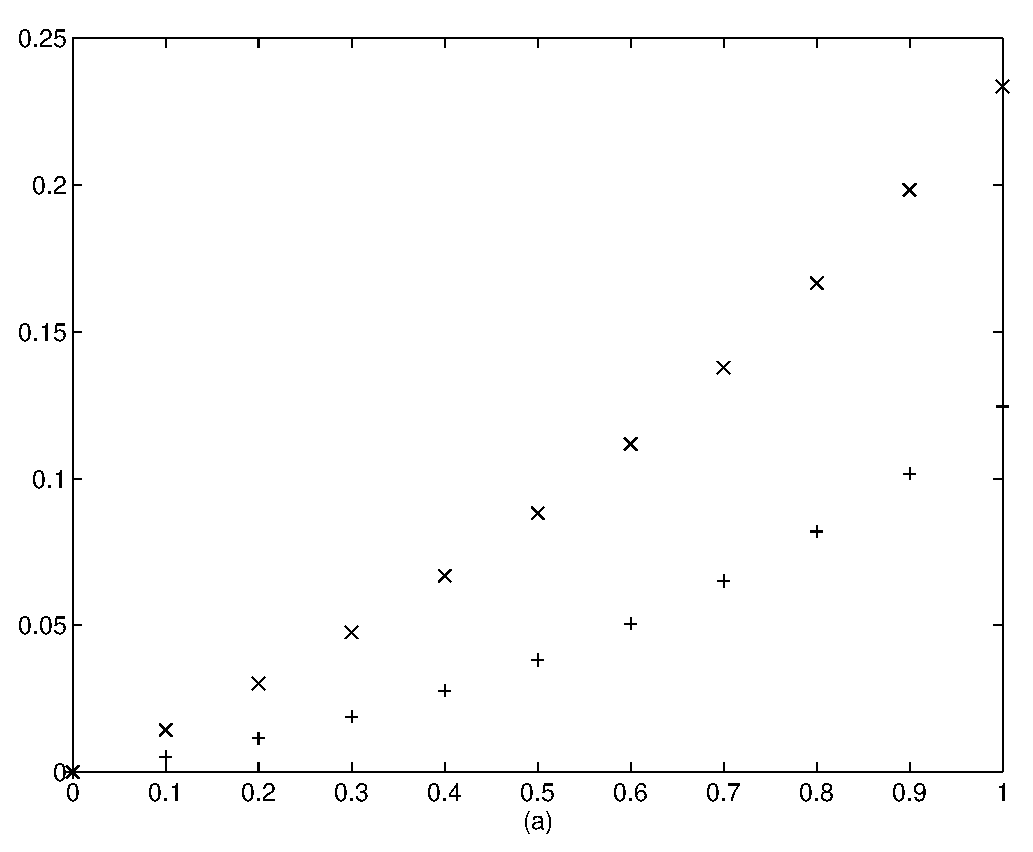
\psfig{file=figures/globerr1.eps,width=2.9in}
   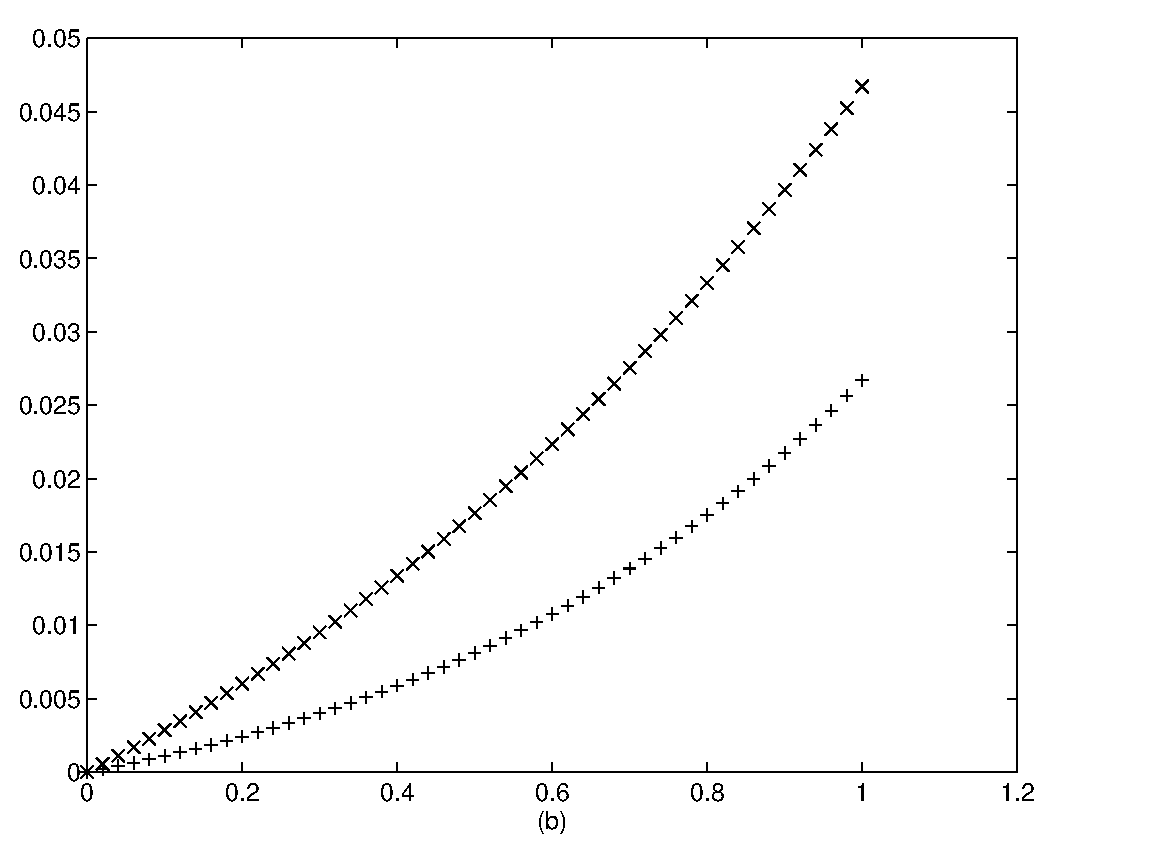
\psfig{file=figures/globerr2.eps,width=3.3in}}
   \caption{Comparison of the global discretization error (marked by
   $+$) with its estimate given in \protect\Ref{eq:globerr} 
   (marked by $\times$) for the step sizes (a) $h=0.1$ and 
   (b) $h=0.02$.}
   \label{fig:globerr1}
\end{figure}

\subsubsection*{Explicit Computation of Error Bounds}
\index{error bound!explicit computation}

Another important consequence of Proposition~\ref{prop:globerr1} is
that it allows us to compute the solution of the initial value
problem \Ref{eq:simplest} on a given interval $[0,T]$ up to a
prescribed accuracy.  Indeed, we just have to use the estimate
\Ref{eq:globerr} on the global discretization error.  

For an illustration of this fact suppose that we want to approximate 
a solution of \Ref{eq:simplest} on the interval $t\in [0,2]$
where the maximal global discretization 
error\index{Euler's method!global discretization error} is less than $0.01$.
It follows from \Ref{eq:globerr} that this is certainly the case if the
step size $h$ is chosen such that
\[
e^2(e^2-1)\frac{h}{2} = 0.01,
\]
or, equivalently,
\[
h = \frac{0.02}{e^2(e^2-1)} \approx 0.000424.
\]
Indeed, if this is the case then we find  with \Ref{eq:globerr}
\[
|\epsilon(k)| \le e^2(e^{kh}-1)\frac{h}{2} \le e^2(e^2-1)\frac{h}{2} = 0.01.
\]
The result of the corresponding \Matlab computation of the global
discretization error is shown in Figure~\ref{fig:globerr2}.
\begin{figure}[htb]
   \centerline{%
   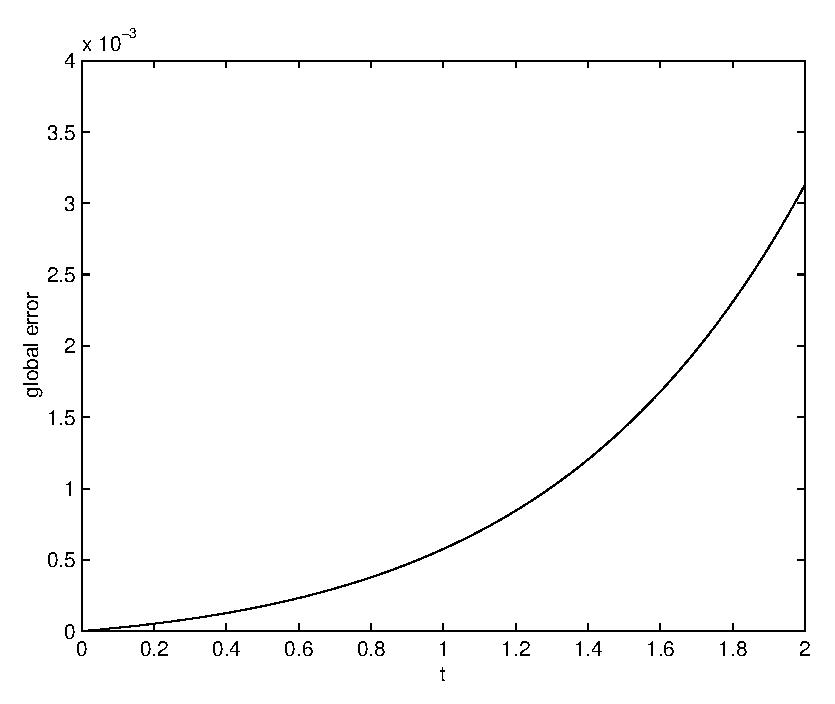
\psfig{file=figures/globerr5.eps,width=3.6in}}
   \caption{The global discretization error for the solution of
   \protect\Ref{eq:simplest} on the interval $[0,2]$ with
   step size $h=0.000424$.}
   \label{fig:globerr2}
\end{figure}



\EXER

\TEXER

\noindent In Exercises~\ref{c15.2.1a} -- \ref{c15.2.1c} compute
bounds on the local and global error for Euler's method applied
to the given initial value problem.  Perform the same steps as in
the treatment of the initial value problem \Ref{eq:simplest} in
the text.
\begin{exercise} \label{c15.2.1a}
$\frac{\dps dx}{\dps dt} = 3x,\quad x(0)=1$.
\end{exercise}
\begin{exercise} \label{c15.2.1b}
$\frac{\dps dx}{\dps dt} = x,\quad x(0)=2$.
\end{exercise}
\begin{exercise} \label{c15.2.1c}
$\frac{\dps dx}{\dps dt} = 3x,\quad x(0)=2$.
\end{exercise}

\begin{exercise} \label{c15.2.2}
Apply the implicit Euler method to the initial value problem
\Ref{eq:simplest}.  Then determine a formula for the local 
discretization error that is analogous to \Ref{eq:locerrdef}.
{\bf Hint:} Before proceeding as for Euler's method solve
for $x_{k+1}$ in \Ref{eq:impleulit} in this specific case.
\end{exercise}

\CEXER

\noindent In Exercises~\ref{c15.2.3a} -- \ref{c15.2.3b}
determine a step size $h$ such that the global discretization error
for the solution of \Ref{eq:simplest} on the given interval using 
Euler's method is less than the given absolute tolerance.  Verify 
your results by a computation of the global discretization error 
using \Matlabp.
\begin{exercise} \label{c15.2.3a}
Interval $[0,4]$ and absolute tolerance $2$.
\end{exercise}
\begin{exercise} \label{c15.2.3b}
Interval $[0,5]$ and absolute tolerance $10$.
\end{exercise}

\begin{exercise} \label{c15.2.4}
Suppose that you want to solve \Ref{eq:simplest} by Euler's
method with a fixed step size $h=0.005$ on the interval $[0,T]$.  
How large can you choose $T$ so that the global discretization
error does not exceed $0.05$?  Confirm your result using \Matlabp.
\end{exercise}

\section{Local and Global Error Bounds}
\label{sec:LGEE}

We now want to analyze the error of a numerical method applied
to an initial value problem of the form
\begin{eqnarray*}
\frac{dx}{dt} & = & f(t,x)\\
 x(t_0) & = & x_0.
\end{eqnarray*}
Before introducing the general concept, we recall the crucial points 
in the error analysis that we have performed in Section~\ref{sec:EEEM}.  

\subsubsection*{Error Analysis From Section~\ref{sec:EEEM}}

We introduced two different types
of error: the {\em local discretization error\/} $\delta(k)$ and the 
{\em global discretization error\/} $\epsilon(k)$.  

For Euler's method, the local error is bounded by
\[
\delta(k)\le \delta_h \le C_E h^2,
\]
where $C_E >0$ is a constant depending on the length of the interval 
$[0,T]$ on which the solution is approximated, see \Ref{eq:locerr}.  
(For example, $C_E =e^T/2$.)  In particular, on the interval
$[0,T]$, the local error goes to zero at least as fast as a 
quadratic function in the step size $h$.

For Euler's method the global error is bounded by
\[
|\epsilon(k)|\le Dh,
\]
with a constant $D>0$ that again just depends on $T$, see 
\Ref{eq:globerr}.  Hence the global error tends to zero at least as fast 
as a linear function in the step size $h$.  Roughly speaking, one power 
is lost going from the local to the global error, and this power is
lost while going through the estimate in \Ref{eq:globest}.  The same
phenomenon occurs in the general error analysis.

\subsection*{A General Form for a Numerical Method}

Let $x(t)$ be the solution of the initial value problem.
From now on we represent an explicit numerical 
method\index{numerical method!explicit} by a function $\Phi$
as follows: for $k=0,1,\ldots,K-1$ we have $t_k=t_0 + kh$, $x_0 = x(t_0)$,
and
\[
x_{k+1} = x_k + h\Phi(t_k,x_k,h).
\]

In Euler's method \Ref{eq:eulmethod}
\[
\Phi(t_k,x_k,h)=f(t_k,x_k).
\]
In particular, in this case, $\Phi$ does not depend on the step size $h$.
In the modified Euler method \Ref{eq:meulmethod}
\[
\Phi(t_k,x_k,h) = \frac{1}{2}
\Big( f(t_k, x_k)+f(t_k+h, x_k + h f(t_k, x_k))\Big).
\]

\subsubsection*{A General Form for Errors}

Next we introduce the two different types of error for a numerical method
given by $\Phi$.
\begin{Def}
\label{def:errors}
\begin{itemize}
\item[(a)] \index{discretization error!local}
The {\em local discretization error\/} $\delta(k+1)$ is defined as
\[
\delta(k+1) = x(t_{k+1}) - (x(t_k) + h\Phi(t_k,x(t_k),h)),
\]
where $k=0,1,\ldots,K-1$.
\item[(b)] \index{discretization error!global}
The {\em global discretization error\/} $\epsilon(k)$ is given by
\[
\epsilon(k) = x(t_k)-x_k, 
\]
where $k=0,1,\ldots,K$.
\end{itemize}
\end{Def}

\subsection*{A Theorem on Global Discretization Errors}

The purpose is to find a bound on the global error by the same 
technique as in Section~\ref{sec:EEEM}.  For this we need two assumptions:
\begin{itemize}
\item[(i)] In the error estimates for Euler's method it was very convenient 
to use a bound for the local error that is independent of the actual 
step $k$.  Hence we assume that there is a constant $\delta_h>0$ such that
\begin{equation} \label{eq:locerrbound}
|\delta(k+1)| \le \delta_h \quad \mbox{for all $k=0,1,\ldots,K-1$.}
\end{equation}
In concrete examples this fact can be guaranteed by the differentiability
of the right hand side $f$ in the initial value problem.
\item[(ii)] We also need an additional assumption on the function $\Phi$:
we assume that there is a constant $L>0$ such that for all $t,h,y,z$
\begin{equation} \label{eq:PhiLip}
|\Phi(t,y,h)-\Phi(t,z,h)|\le L|y-z|.
\end{equation}
For Euler's method $\Phi(t,x,h)=f(t,x)$ and therefore \Ref{eq:PhiLip} is
satisfied if $f$ is (globally) Lipschitz 
continuous\index{Lipschitz continuous} in $x$.
\end{itemize}

We are now in the position to derive a bound for the global 
discretization error proceeding completely analogous to 
Section~\ref{sec:EEEM}.   Observe that by 
Definition~\ref{def:errors}(a)
\[
x(t_k) =  x(t_{k-1}) + h\Phi(t_{k-1},x(t_{k-1}),h)+\delta(k).
\]
On the other hand, the numerical method can be written as
\[
x_k = x_{k-1} + h\Phi(t_{k-1},x_{k-1},h).
\]
Subtracting these two equations from each other and using \Ref{eq:PhiLip},
\Ref{eq:locerrbound} we obtain
\begin{eqnarray*}
|\epsilon(k)| &=& |x(t_k)-x_k|\\
&=& |x(t_{k-1})-x_{k-1} + h[\Phi(t_{k-1},x(t_{k-1}),h)-
\Phi(t_{k-1},x_{k-1},h)]
+\delta(k)|\\
&\le& |x(t_{k-1})-x_{k-1}|+hL|x(t_{k-1})-x_{k-1}|+|\delta(k)|\\
&\le& (1+hL)|x(t_{k-1})-x_{k-1}|+\delta_h\\
&=& (1+hL)|\epsilon(k-1)|+\delta_h.
\end{eqnarray*}
This inequality is of the same type as the inequality in first line in
\Ref{eq:globest} --- one just has to replace the first $h$ by $hL$.
Hence we can repeat the estimate in \Ref{eq:globest} and obtain
\[
|\epsilon(k)| \le \frac{(1+hL)^k -1}{hL}\delta_h.
\]
Since $1+hL\le e^{hL}$ we have proved the following result.
\begin{thm} \label{prop:glerr}
\index{discretization error!global}
\index{error bound}
Suppose that \Ref{eq:locerrbound} and \Ref{eq:PhiLip} hold.  Then the
global discretization error of the numerical method given
by the function $\Phi$ satisfies 
\begin{equation} \label{eq:geestimate}
|\epsilon(k)| \le \left(\frac{e^{khL}-1}{L}\right)\frac{\delta_h}{h}.
\end{equation}
\end{thm}

\subsubsection*{An Example Using Euler's Method}

The estimate \Ref{eq:geestimate} indicates that the constant $L$
plays an important role for the size of the global discretization error.
Indeed, let us illustrate this fact by applying Euler's method to the
initial value problem
\begin{equation} \label{exam:Lchange}
\begin{array}{rcl}
\dps\frac{dx}{dt} & = & \lambda x\\
 x(0) & = & 1,
\end{array}
\end{equation}
on the interval $[0,T]$.
In this case $L=\lambda$ since for Euler's method
\[
|\Phi(t,y,h)-\Phi(t,z,h)|=|f(t,y)-f(t,z)|=|\lambda y-\lambda z|=\lambda |y-z|.
\]
Moreover, since we know the exact solution we may compute 
$\delta_h$ for this case as follows: we have
\[
\delta(k+1) = e^{\lambda t_{k+1}} - (e^{\lambda t_k} + 
\lambda h e^{\lambda t_k}) = e^{\lambda kh}(e^{\lambda h}-(1+\lambda h)),
\]
and since $e^{\lambda h}-(1+\lambda h)\le 
e^{\lambda h}\frac{(\lambda h)^2}{2}$ we obtain (see also \Ref{eq:locerr})
\[
\delta(k+1)\le e^{\lambda kh} e^{\lambda h}\frac{(\lambda h)^2}{2}\le 
e^{\lambda T}\frac{(\lambda h)^2}{2}.
\]
Therefore we can choose 
\begin{equation} \label{eq:dhlam}
\delta_h = \lambda^2 e^{\lambda T} \frac{h^2}{2}.
\end{equation}
In fact, observe that for $\lambda=1$ we recover \Ref{eq:euldh}.

Proceeding as in Section~\ref{sec:EEEM} we set $\lambda =2$ and
compute the global
discretization error\index{Euler's method!global discretization error} 
and its bound in \Ref{eq:geestimate} by
\Matlab on the interval $[0,1]$ for the step size $h=0.1$.  
Concretely we type
\begin{verbatim}
h      = 0.1;
L      = 2;
t(1)   = 0;
x(1)   = 1;
err(1) = 0;
est(1) = 0;
K      = 1/h;
for k = 1:K
     t(k+1) = t(k)+h;
     x(k+1) = (1+L*h)*x(k);
   err(k+1) = exp(L*t(k+1))-x(k+1);
   est(k+1) = exp(L)*(exp(L*k*h)-1)*L*h/2;
end
plot(t,err,'+')
hold on
plot(t,est,'x')
\end{verbatim}
The result is shown in Figure~\ref{fig:Lgeest}.  A comparison with
Figure~\ref{fig:globerr1} shows that the error is indeed significantly bigger
reflecting the fact that here $L=2$ whereas in the example in 
Section~\ref{sec:EEEM} this constant was one.

\begin{figure}[htb]
   \centerline{%
   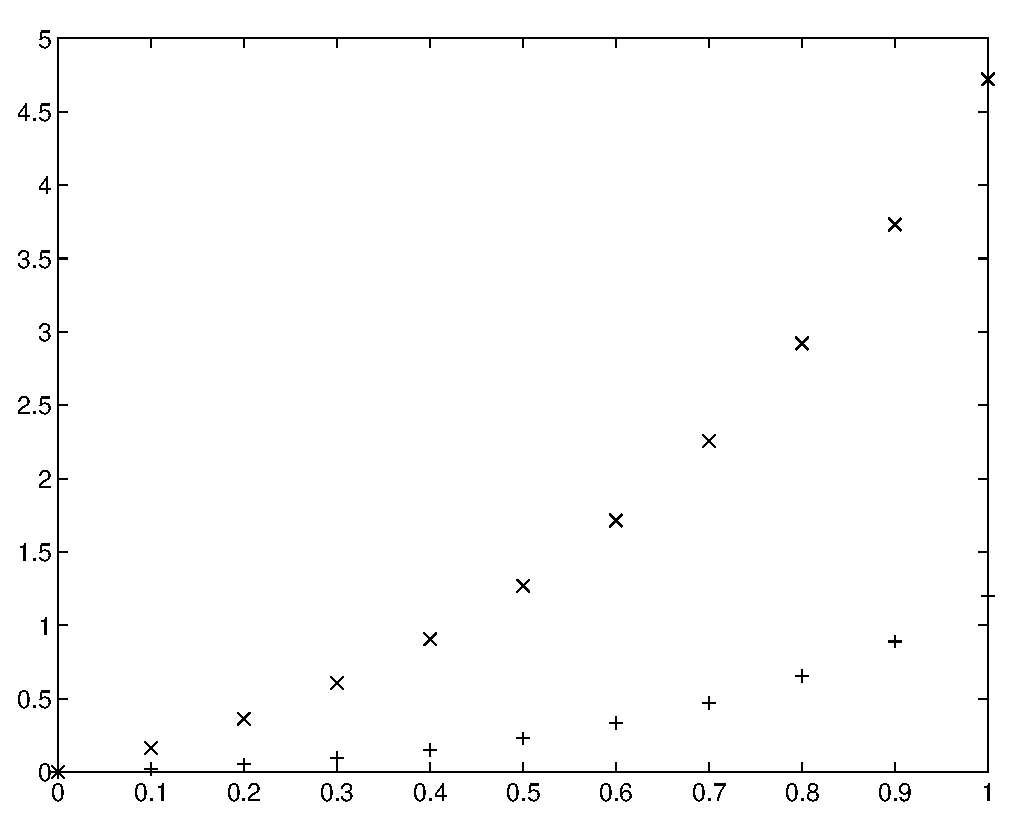
\psfig{file=figures/globerr3.eps,width=3.2in}}
   \caption{The global discretization error (marked by
   $+$) and its bound given in \protect\Ref{eq:geestimate}
   (marked by $\times$) for the step size $h=0.1$.}
   \label{fig:Lgeest}
\end{figure}

\subsection*{A Bound on Local Discretization Errors}
\index{error bound}

It remains to demonstrate how to determine a bound $\delta_h$ on
the local discretization error $\delta(k)$ for a given numerical 
method applied to the initial value problem
\begin{eqnarray*}
\frac{dx}{dt} & = & f(t,x)\\
x(t_0) & = & x_0,
\end{eqnarray*}
on the interval $[t_0,t_e]$.  Again we consider Euler's method.
The crucial tool for the computation of the local error is a Taylor
expansion of the solution combined with the fact that the 
derivatives of $x(t)$ can be written in terms of the function $f$
by the differential equation.  Using this idea we 
expand $x(t_{k+1})=x(t_k+h)$ up to second order by
\begin{eqnarray*}
x(t_{k+1})&=&
x(t_k)+h\frac{dx}{dt}(t_k)+\frac{h^2}{2}\frac{d^2x}{dt^2}(t_k+\theta h)\\
&=& x(t_k)+hf(t_k,x(t_k))+\frac{h^2}{2}\frac{d^2x}{dt^2}(t_k+\theta h),
\end{eqnarray*}
with an appropriate $0<\theta<1$.  Substitution into the expression
for the local error leads to
\begin{eqnarray*}
\delta(k+1)&=&x(t_{k+1}) - (x(t_k) + hf(t_k,x(t_k)))\\
&=& \frac{h^2}{2}\frac{d^2x}{dt^2}(t_k+\theta h).
\end{eqnarray*}
Hence, choosing a constant $C_E$ by
\[
C_E=\frac{1}{2}
\max\left\{ \left\vert\frac{d^2x}{dt^2}(s)\right\vert,\, t_0\le s\le t_e\right\},
\]
we find that $\delta(k+1)\le \delta_h$ for all $k$ if we set
\[
\delta_h = C_E h^2.
\]

Since the solution $x(t)$ of the initial value problem is in general
not known, it is more appropriate to find a bound for the
constant $C_E$ directly from the right hand side
$f$ in the differential equation.  We now outline a procedure
how this can be accomplished.

We have $\frac{dx}{dt}(t)=f(t,x(t))$ and it follows
\arraystart
\begin{equation}
\label{eq:Taylor2}
\begin{array}{rcl}
\dps\frac{d^2x}{dt^2}(t) &=& \dps\frac{\partial f}{\partial t}(t,x(t))
+\frac{\partial f}{\partial x}(t,x(t))\frac{dx}{dt}(t)\\
&=& \dps\frac{\partial f}{\partial t}(t,x(t))
+\frac{\partial f}{\partial x}(t,x(t))f(t,x(t)).
\end{array}
\end{equation}
\arrayfinish
Hence if a solution has to be computed for $t_0\le t\le t_e$, and the
values of the solution certainly are in the range $x_\ell \le x \le x_u$, then
\begin{equation} \label{eq:CE}
C_E\le \frac{1}{2}\max\left\{ \left\vert\frac{\partial f}{\partial t}(s,y)
+\frac{\partial f}{\partial x}(s,y)f(s,y)\right\vert,\, t_0\le s\le t_e,\quad
x_\ell \le y \le x_u \right\}.
\end{equation}

As an example of \Ref{eq:CE} we approximate the solution of the initial 
value problem
\begin{eqnarray*}
\frac{dx}{dt} & = & 5 x\\
 x(0) & = & 1,
\end{eqnarray*}
on the interval $[0,T]$.  Here $f(t,x)=5 x$ and therefore
\[
\frac{\partial f}{\partial t}(t,x)=0\AND
\frac{\partial f}{\partial x}(t,x)=5.
\]
From the ODE we see that the solution is monotonically increasing
and thus we find that
\[
C_E\le \frac{1}{2}\max\left\{ \left\vert 0+5\cdot 5y\right\vert,
y=x(T) \right\} = \frac{25}{2}x(T).
\]
Therefore we can choose
\[
\delta_h = \frac{25}{2}\bar x h^2
\]
for any $\bar x$ such that $\bar x \ge x(T)$.  In particular,
we have confirmed the result we have previously obtained, 
see \Ref{eq:dhlam}.

The computation of the local discretization error using Taylor expansions 
is quite tedious.  Therefore we just remark here that
for the modified Euler 
method\index{modified Euler method!local discretization error} 
the local error can be bounded by a function
of the form
\[
\delta_h = C_Mh^3,
\]
and for the fourth order Runge-Kutta 
method\index{fourth order Runge-Kutta method!local discretization error} 
\index{Runge-Kutta method!fourth order!local discretization error} 
the local discretization error is bounded by
\[
\delta_h = C_R h^5.
\]
Here $C_M$ and $C_R$ are positive constants.  

\subsection*{A Bound on Global Discretization Errors}

Once the local discretization error is bounded we can use
Theorem~\ref{prop:glerr} to obtain a bound on global discretization 
error.  In particular, we can prove:
\begin{prop} \label{prop:errEMR}
Suppose that \Ref{eq:PhiLip} holds.  Then there are constants $C_E$,
$C_M$ and $C_R$ such that the global discretization error of
\begin{itemize}
\item[(a)] \index{Euler's method!global discretization error}
Euler's method is bounded by
\[
|\epsilon(k)| \le \frac{e^{khL}-1}{L}C_E h;
\]
\item[(b)] \index{modified Euler method!global discretization error}
the modified Euler method is bounded by
\[
|\epsilon(k)| \le \frac{e^{khL}-1}{L}C_M h^2;
\]
\item[(c)] \index{fourth order Runge-Kutta method!global discretization error}
\index{Runge-Kutta method!fourth order!global discretization error} 
the fourth order Runge-Kutta method is bounded by
\[
|\epsilon(k)| \le \frac{e^{khL}-1}{L}C_R h^4.
\]
\end{itemize}
\end{prop}

In view of this proposition it is clear that the fourth order Runge-Kutta 
method is much better than Euler's method or the modified
Euler method: the reason is that for small step sizes $h$ the value of 
$h^4$ is much smaller than $h^2$ or even $h$ itself.  Hence the
global discretization error of the fourth order Runge-Kutta method is,
for reasonably small step sizes, much smaller than for the other two
methods.  In addition, it is also evident how the {\em fourth order\/} 
Runge-Kutta method got its name.

\subsubsection*{Specifying the Tolerance}

In principle, we can use Proposition~\ref{prop:errEMR} to find a step 
size for which the global discretization error is not bigger than a
specified tolerance.  To illustrate this point,  
consider the initial value problem (see also \Ref{eq:eulexivp})
\begin{eqnarray*}
\frac{dx}{dt} & = & x+t \\
x(1) & = & 2.
\end{eqnarray*}
The aim is to find a step size $h$ such that Euler's method is
approximating the solution on the interval $[1,3]$ up to a global 
discretization error smaller than $0.1$.  By Proposition~\ref{prop:errEMR}
this can be guaranteed if $h$ is chosen so that
\[
\frac{e^{khL}-1}{L}C_E h < 0.1.
\]
For this example $L=1$, since
\[
|y+t-(z+t)|=|y-z|=1\cdot |y-z|.
\]

We now find a bound for the constant $C_E$.  We compute
\[
\frac{\partial f}{\partial t}(s,y)=\frac{\partial f}{\partial x}(s,y)=1.
\]
We see from the ODE that the solution is monotonically increasing.
Suppose that we know that for $t\in [1,3]$ the solution $x(t)$ is bounded
by $40$ from above.  Using \Ref{eq:CE} we obtain an estimate for $C_E$ by
\[
C_E\le \frac{1}{2}\max\left\{\vert 1+1\cdot f(s,y)\vert,\, 1\le s\le 3,\,
2 \le y \le 40 \right\}=\frac{44}{2}=22.
\]
Since $e^{kh}\le e^{t_e-t_0}=e^2$, we can choose an $h$ such that
\[
(e^2-1)22h < 0.1\quad \Longleftrightarrow 
\quad h<\frac{1}{220(e^2-1)}\approx 0.00071.
\]
Indeed, computing a solution with \Matlab by
\begin{verbatim}
h     = 0.0007;
t(1)  = 1;
x(1)  = 2;
K     = round(2/h);
for k = 1:K
     t(k+1) = t(k)+h;
     x(k+1) = x(k)+h*(x(k)+t(k));
end
plot(t,x)
xlabel('t')
ylabel('x')
\end{verbatim}
we obtain the result in Figure~\ref{fig:hsmall}.  (The \Matlab
command {\tt round} rounds a number towards the nearest integer.)
The outcome cannot be distinguished from the exact solution shown 
in Figure~\ref{fig:eulex1}(b).

\begin{figure}[htb]
   \centerline{%
   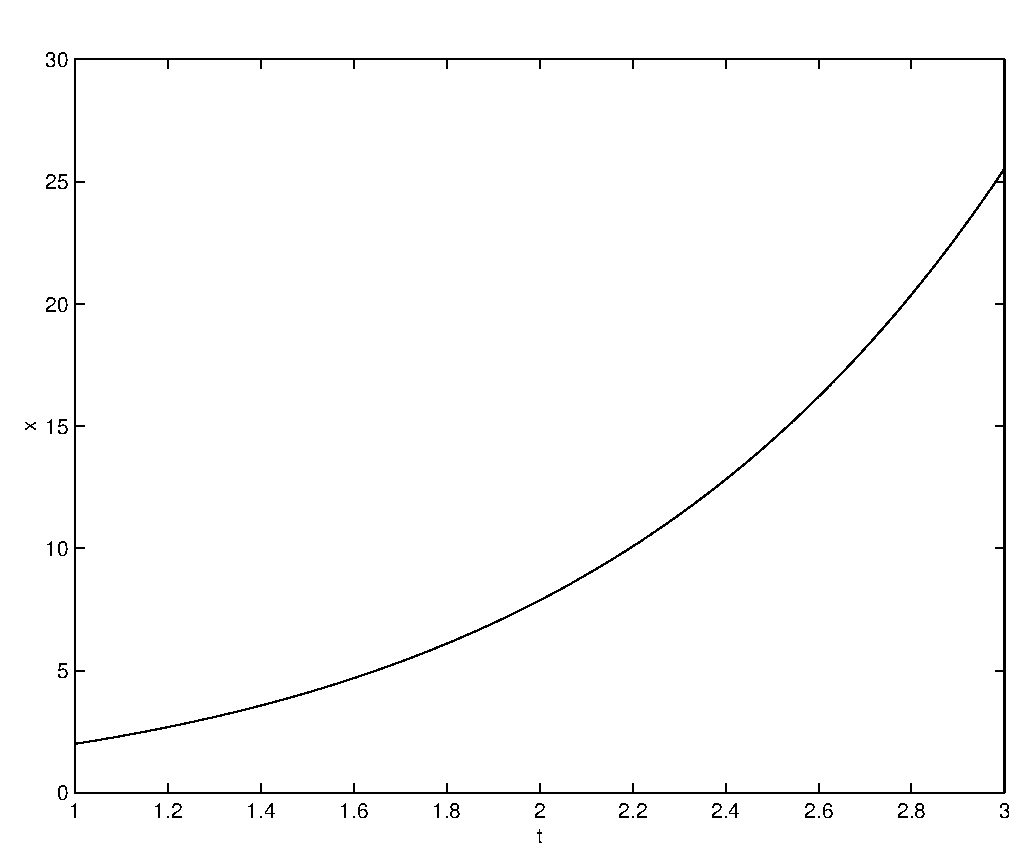
\psfig{file=figures/globerr6.eps,width=3.2in}}
   \caption{The numerical solution obtained by Euler's method for the 
   step size $h=0.0007$.}
   \label{fig:hsmall}
\end{figure}

\EXER

\TEXER

\begin{exercise} \label{c15.3.1}
Determine the function $\Phi=\Phi(t_k,x_k,h)$ which belongs to the 
fourth order Runge-Kutta method.
\end{exercise}

\noindent In Exercises~\ref{c15.3.2a} -- \ref{c15.3.2b} find an estimate
for the constant $C_E$ of the form $C_E \le Kx(t_0)$ where $x(t)$ is the
solution of the specified initial value problem on $[0,T]$ and $t_0\in[0,T]$.
\begin{exercise} \label{c15.3.2a}
$\dps\frac{dx}{dt} = 3 x$ where $x(0) = 2$.
\end{exercise}
\begin{exercise} \label{c15.3.2b}
$\dps\frac{dx}{dt} = -x$ where $x(0) = 1$.
\end{exercise}


\CEXER

\begin{exercise} \label{c15.3.3}
Set $\lambda=0.2$ and the step size $h=0.1$.  Use \Matlab to compute 
the global discretization error and its bound in \Ref{eq:geestimate}
on the interval $[0,1]$.  Compare the result with the ones obtained 
in Figures~\ref{fig:globerr1} and \ref{fig:Lgeest}.
\end{exercise}



\section{Appendix: Variable Step Methods}
\label{sec:appslc}

The idea underlying variable step methods is to perform {\em step 
length controls\/}\index{step length control} rather than using steps of 
fixed length.   The strategy is to vary the step size in each step of the 
integration so that a fixed error bound is always maintained.   

More concretely, suppose that we can estimate in step $k$ the error that is
made in the numerical solution.  Then we can use this estimate to find
an appropriate step size $h_{k+1}$ for the next step.  This principle has
the advantage that large step sizes are used when the error bound
is small and small step sizes are used when the error bound is large.
The \Matlab command {\tt ode45}\index{\computer!ode45}
is based on explicit Runge-Kutta methods and it uses step length 
control to solve initial value problems 
numerically\index{initial value problem!numerical solution}.

Rather than explaining step length control mechanisms in detail
we give an example illustrating such a mechanism used in
{\tt ode45}.  Consider the initial value problem
\arraystart
\begin{equation*}  \label{eq:odestepivp}
\begin{array}{rcl}
\dps \frac{dx}{dt}(t) & = & -e^{10t}x^2 \\
 x(0) & = & 3.
\end{array}
\end{equation*}
\arrayfinish
Store the right hand side in the m-file {\tt f18\_4\_1.m}
\begin{verbatim}
function f = f18_4_1(t,x)
f = -exp(10*t)*x*x;
\end{verbatim}
and compute an approximation of the solution on the interval
$t\in[0,1.2]$:
\begin{verbatim}
[t,x] = ode45('f18_4_1',[0 1.2],3);
plot(t,x)
xlabel('t')
ylabel('x')
\end{verbatim}\index{\computer!ode45}
The result is shown in Figure~\ref{fig:ode45step}(a).
In particular, note that the solution is almost linear
for $t\in[0,0.2]$ and indistinguishable from zero for $t>0.8$.
Since the behavior of linear functions is easy to predict, we expect
that the step length control\index{step length control}
mechanism in {\tt ode45} will lead
to larger step sizes in those intervals.  To look at the step
lengths we will have to compute the differences of the consecutive
entries in {\tt t}.  In \Matlab this can be done with the
command {\tt diff}\index{\computer!diff}.  Typing
\begin{verbatim}
dt  = diff(t);
tdt = t(2:length(t));
plot(tdt,dt,'o')
xlabel('t')
ylabel('step lengths')
\end{verbatim}\index{\computer!length}
we obtain the result shown in Figure~\ref{fig:ode45step}(b).
At the beginning of the numerical solution -- within the region
where the solution shows almost linear behavior -- the step sizes
are quite large. Then the step sizes decrease until the almost constant
part is detected by the step length control mechanism and the step
sizes\index{step size} increase again.
At the end the step size becomes smaller, since  the
numerical approximation ends at $t_e = 1.2$ and
the step sizes have to be adjusted to this value.
Altogether {\tt ode45}\index{\computer!ode45}
qualitatively behaves as expected.

\begin{figure}[htb]
   \centerline{%
   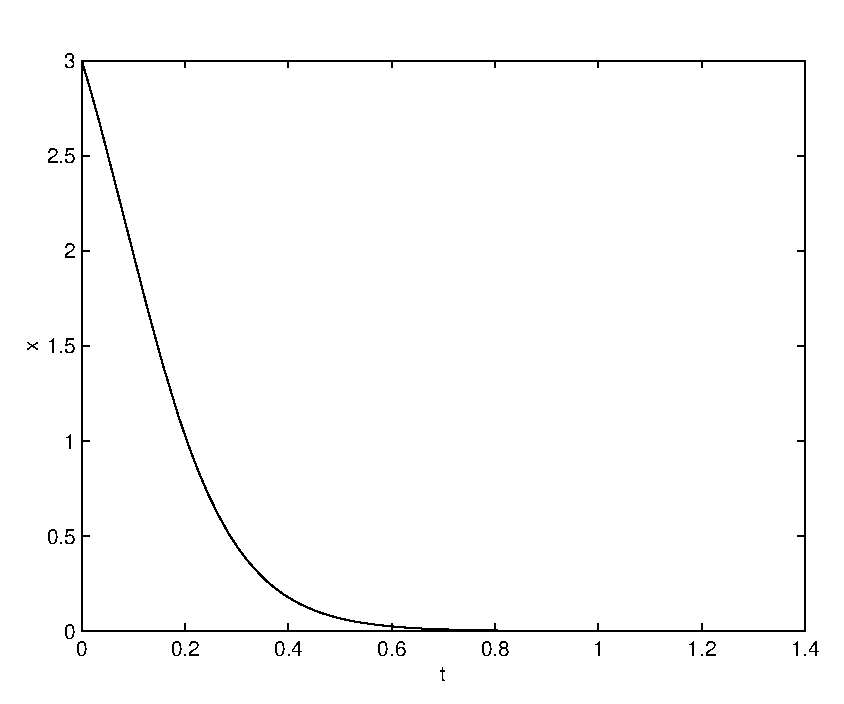
\psfig{file=figures/ode45step1.eps,width=3in}
   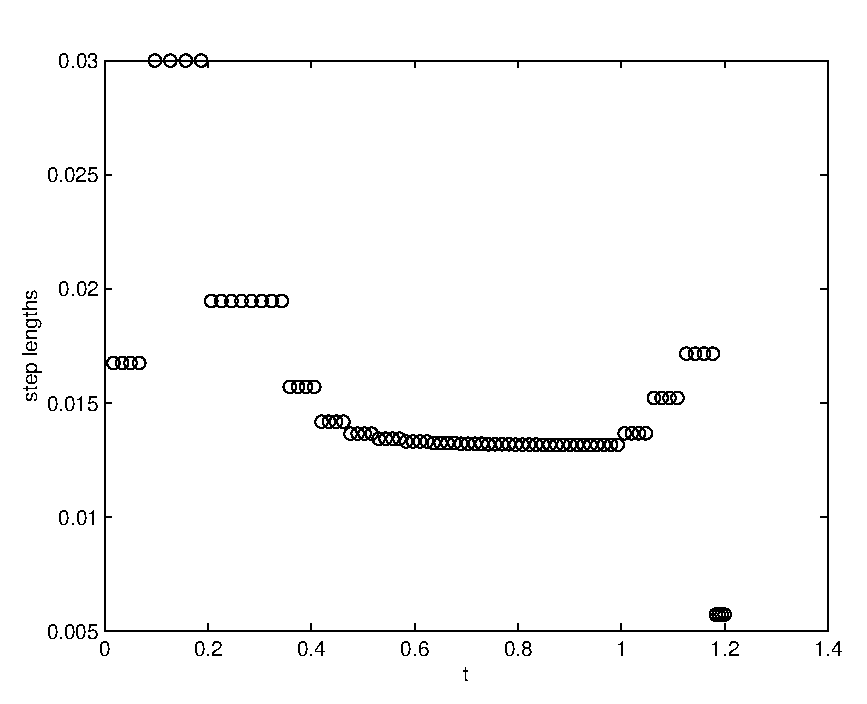
\psfig{file=figures/ode45step2.eps,width=3in}}
   \caption{(a) Numerical solution of the initial value problem
   \protect\Ref{eq:odestepivp} using {\tt ode45};
   (b) the different step sizes used by {\tt ode45} in
   the numerical approximation.}
   \label{fig:ode45step}
\end{figure}
\end{document}
